%% BioMed_Central_Tex_Template_v1.06    %
%%                                      %

% Multi-subject/DLA EMG-based control of mechanical hands
% Castellini, Fiorilla, Sandini
%
% Submitted to J NeuroEng Rehab, November, 2008

\NeedsTeXFormat{LaTeX2e}[1995/12/01]
\documentclass[10pt]{bmc_article}    

\usepackage{cite} % Make references as [1-4], not [1,2,3,4]
\usepackage{url}  % Formatting web addresses  
\usepackage{ifthen}  % Conditional 
\usepackage{multicol}   %Columns
\usepackage[utf8]{inputenc} %unicode support
\usepackage{amsmath}
\usepackage[psamsfonts]{amssymb}
\usepackage{graphicx}
\urlstyle{rm}
 
\def\includegraphic{}
%\def\includegraphics{}

\setlength{\topmargin}{0.0cm}
\setlength{\textheight}{21.5cm}
\setlength{\oddsidemargin}{0cm} 
\setlength{\textwidth}{16.5cm}
\setlength{\columnsep}{0.6cm}

\newboolean{publ}

%Review style settings
\newenvironment{bmcformat}{\begin{raggedright}\baselineskip20pt\sloppy\setboolean{publ}{false}}{\end{raggedright}\baselineskip20pt\sloppy}
%Publication style settings
%\newenvironment{bmcformat}{\fussy\setboolean{publ}{true}}{\fussy}

\def\RR{\mathbb{R}}
\def\NN{\mathbb{N}}
\def\xx{\mathbf{x}}
\def\yy{\mathbf{y}}
\def\ww{\mathbf{w}}

\begin{document}

\begin{bmcformat}

\title{Multi-subject / Daily-Life Activity\\EMG-based control of mechanical hands}
 
\author{%
  Claudio Castellini\correspondingauthor$^1$%
  \email{Claudio Castellini - claudio.castellini@unige.it}%
\and
  Angelo Emanuele Fiorilla$^{2,3}$%
  \email{Angelo Emanuele Fiorilla - emanuele.fiorilla@iit.it}%
\and
  Giulio Sandini$^3$%
  \email{Giulio Sandini - giulio.sandini@iit.it}%
}%

\address{%
    \iid(1)LIRA-Lab, University of Genova, viale F. Causa 13, 16145 Genova, Italy\\
    \iid(2)DIST, University of Genova, viale F. Causa 13, 16145 Genova, Italy\\
    \iid(3)Italian Institute of Technology, via Morego 30, 16163 Genova, Italy
}%

\maketitle

\begin{abstract}

\paragraph*{Background:}
in previous work \cite{2008.ICRA,2008.BioCyb}
forearm surface electromyography (EMG) has been effectively used to
control in position \emph{and force} a dexterous mechanical hand, thus laying the basis of
EMG-based control of polyarticulate hand prostheses, such as, e.g.,
Touch Bionics's i-LIMB hand.
So far, the analysis has been concerned with one subject only, fully
able-bodied, and in highly controlled conditions, i.e., with the arm
relaxed and still on a table. In this paper we we describe the outcome of a similar experiment, in which however $10$ healthy subjects participated,
who were left free to walk, raise their hands and arms, sit
down and stand up, etc., as a patient is supposed to do during
Daily-Life Activities. We also propose a cross-subject model analysis, i.e., training a model on a subject and testing it on another one, which reveals that a certain degree of cross-subject compatibility is present.
      
\paragraph*{Results:}
machine learning techniques such as Support Vector Machines (SVMs) are able to achieve excellent results also in this less controlled situation. In particular, in the DLA situation, an average accuracy of about $95\%$ in classification of grip posture is attained, and reconstruction of the required force is obtained with an average correlation factor of $0.90$.

\paragraph*{Conclusions:}
EMG can control in position and force a dexterous mechanical hand and/or a hand prosthesis for any healthy subject, and in DLA situation. Also, there are strong hints that a ``common'' model can be built and shipped along with the prosthesis (rather than having to train it from
scratch), thus shortening the patient's training time.

\end{abstract}

\ifthenelse{\boolean{publ}}{\begin{multicols}{2}}{}

\section*{Background}
\label{sec:introduction}

In recent years rehabilitation medicine, and prosthetics in
particular, has benefited from the advances in mechatronics, a field
which has so far pertained to robotics. This synergy is driving
rehabilitation medicine to a scenario in which an amputee's life will
be better, when more dexterous and controllable prostheses will make
it to the market. The paradigmatic example is represented by the
recent commercialisation of Touch Bionics's i-LIMB prosthetic hand
\cite{ilimb}, which is lightweight, long-running, it has five fingers
and five Degrees-Of-Freedom (DOFs --- one per finger, see Figure
\ref{fig:hands} $(a)$). (At the time of writing, a few hundreds i-LIMBs
have been implanted and sold.)

The dexterity of this prosthesis is very high, though still far from
the best non-prosthetic robot hand prototypes (e.g., the DLR-II hand,
see \cite{Hua2006} and Figure \ref{fig:hands} $(b)$). In fact, it
represents a real breakthrough with respect to the state-of-the-art
commercial prostheses, namely Otto Bock's SensorHand Speed (see Figure
\ref{fig:hands} $(c)$), which has one open/close DOF. Notice, anyway,
that both prostheses still allow for no control of the \emph{force}
required by the patient.

In fact, control is, in general, far from optimal. The most widely
used control device nowadays is surface electromyography (EMG), a
cheap, non-invasive technique by which surface electrodes gather from
the patient's stump skin the (residual) muscle activation potentials
(see, e.g., \cite{deluca}); these potentials are then somehow
translated to motor commands. The current EMG-based strategies employ
large muscles, such as the wrist flexor and extensor, to control one
or, at best, two DOFs (e.g., opening and closing of the Otto Bock's
claw). This means that controlling the prosthesis is highly
non-natural, and implies a long training time for the patient, that
is, the patient must learn how to order the hand what she/he wants it
to do.

Even a dexterous hand prosthesis as the i-LIMB cannot be controlled in
a fine and natural way; it uses two EMG electrodes in combination, to
produce a set of predefined grasp shapes; and the force involved in
the grasp is not controlled. Most of the adaptability is left to the
compliance of the hand itself. Notice that \emph{force control} is a
paramount requirement in Daily-Life Activities (DLA): picture the
possibility of holding an egg without breaking it, or holding a hammer
without letting it slip.

Indeed, as more advanced hand prostheses appear on the market, there
is a strong demand for \emph{accurate control strategies}. This paper
fits in this line of research, showing that plain, old-fashioned EMG,
together with \emph{machine learning} techniques, can be used in a
radically better way to control a dexterous hand prosthesis. In
\cite{2008.ICRA,2008.BioCyb} we have shown that ten EMG electrodes
could enable a healthy human subject to control \emph{in position and
in force} a dexterous mechanical hand such as the DLR-II hand. Here we
carry on the analysis, extending it to $10$ healthy subjects and
showing that the same excellent results are obtained, regardless of
the subject involved; moreover, we relax the highly controlled
conditions of the previous experiment (the subject would keep her/his
arm and body posture rigorously relaxed and still) and show that the
same technique, applied to subjects who can freely move, walk, sit,
raise and lower their arms and pronate/supinate their forearms,
obtains only slightly worse results, which would most likely become
optimal in an online environment.

Our research aims at realising \emph{adaptive prosthetics}, that is,
the possibility for the prosthesis to adapt to the patient's needs and
style: so far, it is the patient that has to adapt to the prosthesis,
and learn how to use it. In our vision, the patient and the prosthesis
are involved in a \emph{reciprocal learning} loop. The result is that
the patient needs less time to correctly use the prosthesis, and also
that she/he can use it in a finer way, more suited to real DLAs. The
results presented in this paper show that this is possible. The final
question remains of whether an
\emph{amputee} can do the same; some initial results seem to indicate
that the answer is positive (see the ``Discussion and conclusions''
section for more details).

The paper is structured as follows: Section \ref{sec:m&ms} introduces
the materials and methods used for the experiments; Section
\ref{sec:exp} presents a detailed analysis of the gathered data, and
the results of it; lastly, in Section \ref{sec:discussion} we discuss
the results and draw a few conclusions.

\section*{Methods}
\label{sec:m&ms}

\subsection*{Subjects and electrode placement}

The experiment was carried out on ten healthy subjects, two women and
eight men, nine right-handed and one left-handed, of an average age of
$30.9 \pm 8.45$ years. The subjects were given no knowledge of what
the experiment was about. We placed on each subject's dominant forearm
$7$ surface EMG electrodes, according to this anatomic guideline:

\begin{itemize}

  \item on the forearm ventral side: near the wrist, above the
    \emph{flexor pollicis longus}; centrally, above the \emph{flexor
    digitorum superficialis}; near the elbow, above the \emph{flexor
    digitorum profundus}; and near the wrist, above the \emph{flexor
    digitorum superficialis} again;

  \item on the forearm dorsal side: near the wrist, above the
    \emph{extensor pollicis brevis / abductor pollicis longus};
    centrally, above the \emph{extensor digitorum communis} and
    \emph{extensor digiti minimi}.

\end{itemize}

These positions were chosen, according to the medical literature
\cite{Kendall},
as carefully as possible in order to identify the best EMG sources and
to detect the activity of the most relevant flexor and extensor
muscles of the forearm. It must be noted, however, that we detected,
both visually and by palpation, that inter-arm differences are
remarkable, depending on the subjects' age, gender and physical
fitness. Moreover, some of the aforementioned muscles are deep into
the forearm, so that muscle cross-talk cannot be avoided. This is a
well-known problem in the EMG literature (\cite{deluca,zecca}) and is
one of the factors that make our problem hard: it is like
reconstructing a coherent speech by listening to $19$ people who talk
at the same time, and not necessarily the ones we want to listen to
are the loudest and clearest speakers in the room.

\subsection*{Sensors and hardware}

%\begin{figure*}[!t] \centering
%  \begin{tabular}{ccc}
%    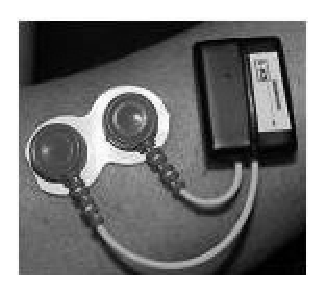
\includegraphics[height=0.16\textheight]{Electrode.eps} &
%    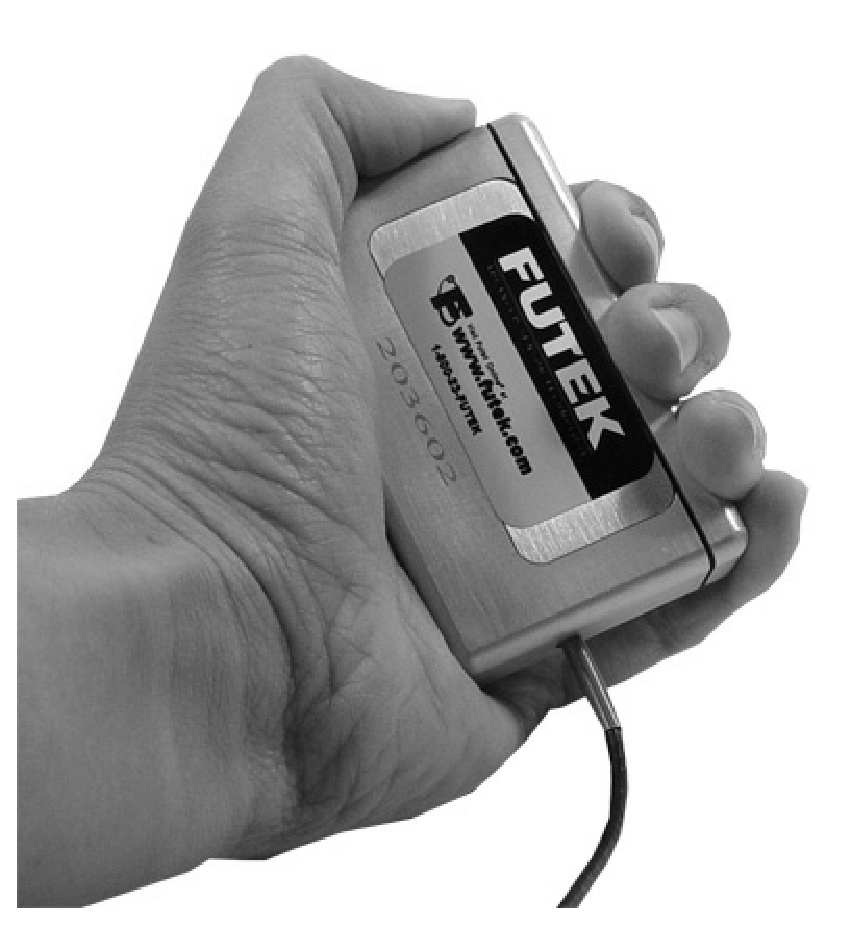
\includegraphics[height=0.16\textheight]{Hand_Gripper.eps} &
%    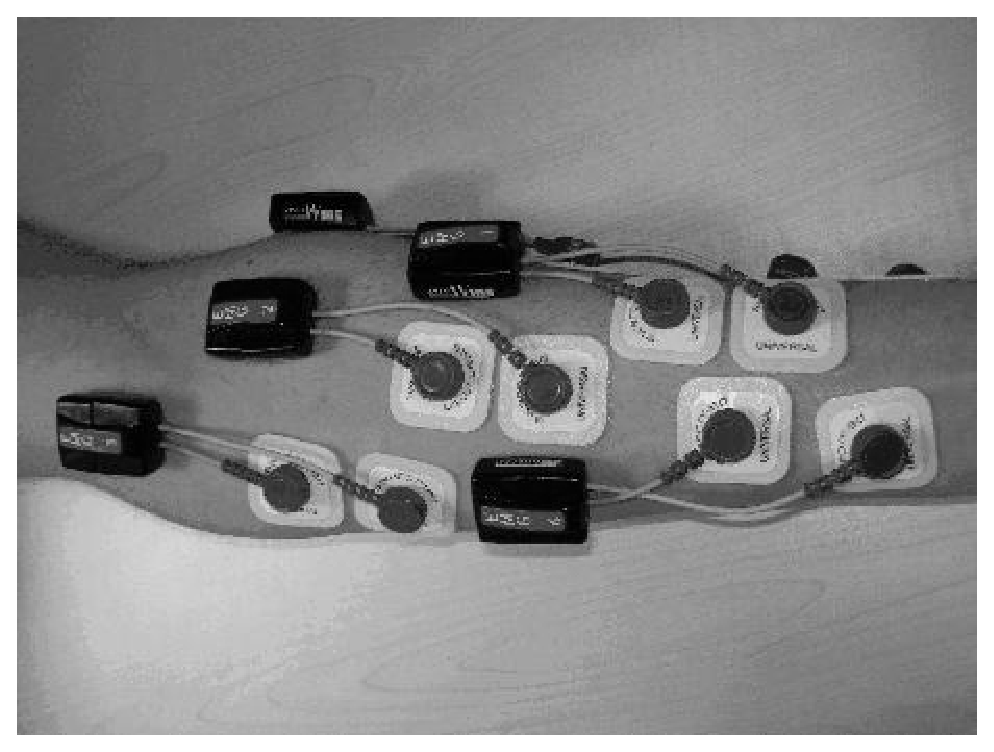
\includegraphics[height=0.16\textheight]{El_Arrangement.eps} \\
%    $(a)$ & $(b)$ & $(c)$ \\
%  \end{tabular}
%  \caption{The experimental setup (\textit{subject side}): $(a)$ an EMG
%    wireless electrode; $(b)$ the FUTEK force sensor; $(c)$ the typical
%    placement of the EMG electrodes on a subject's forearm (ventral side).}
%  \label{fig:SubjSetup}
%\end{figure*}

The electrodes we employed are Aurion ZeroWire wireless surface EMG
electrodes (see \cite{zerowire}). The use of wireless electrodes is
particularly appreciated in such kind of experiments, since the
subjects would eventually have to be free to perform DLA-like actions
during the experiment, i.e., in a specific phase of the experiment
they were allowed to walk around, pronate and supinate their forearms,
sit down and stand up, walk, etc. Wireless electrodes let the subjects
feel free.

Each subject was also given a FUTEK LMD500 Hand Gripper force sensor
(see \cite{LMD500}) in order to detect the force applied by the subjects'
hand during the experiment.

Figure \ref{fig:SubjSetup} shows $(a)$ a single electrode, glued to
the subject's forearm skin; $(b)$ the force sensor as gripped during a
power grasp; and $(c)$ the typical placement of the electrodes
(ventral side of the forearm).

It is well-known that the EMG raw signal relevant bandwidth lies
between $15$ and $500$Hz, so we set the sampling rate at $2$KHz. In
order to avoid synchronisation problems, the same sampling rate was
applied to the force sensor, although we obviously expect a much lower
bandwidth from this sensor than from the EMG sensors.

We used a standard National Instruments data acquisition board
(NI-USB6211) to record the sensors' signals, connected to the receiver
of the EMG wireless device (Figure \ref{fig:ExpSetup}) and to an
amplifier connected to the force sensor. The board was connected via a
USB port to an entry-level laptop. We used a custom National
Instruments' LabView VI block to acquire the signals.

%\begin{figure*}[!t] \centering
%  \begin{tabular}{cc}
%    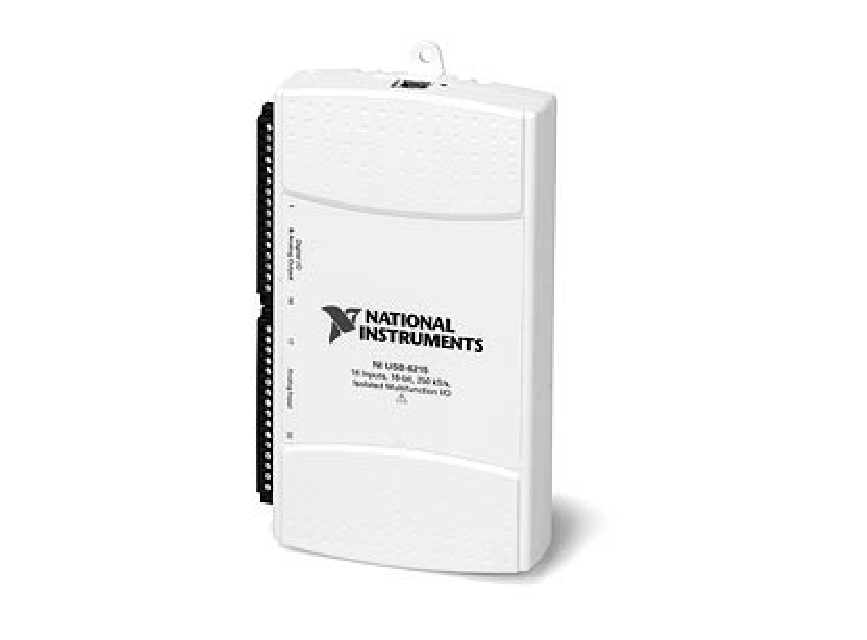
\includegraphics[height=0.16\textheight]{NI-6211.eps} &
%    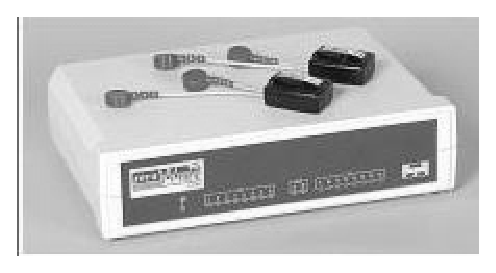
\includegraphics[height=0.16\textheight]{Zero_Base.eps} \\
%  $(a)$ & $(b)$\\
%  \end{tabular}
%  \caption{The experimental setup (\textit{experimenter side}): $(a)$
%   the USB data acquisition card (NI-USB6211); $(b)$ the EMG device
%   receiver.}
%  \label{fig:ExpSetup}
%\end{figure*}

\subsection*{Experiment design}

The experiment consisted of two phases, one right after the
other.

During phase $1$ the subject would keep her/his arm still and relaxed
on a table, and was asked to grasp the force sensor using, in turn,
three different grips (Figure~\ref{fig:Grasps}):

\begin{itemize}
  \item index precision grip;
  \item other fingers precision grip;
  \item power grasp.
\end{itemize}

%\begin{figure*}[!t] \centering
%  \begin{tabular}{ccc}
%    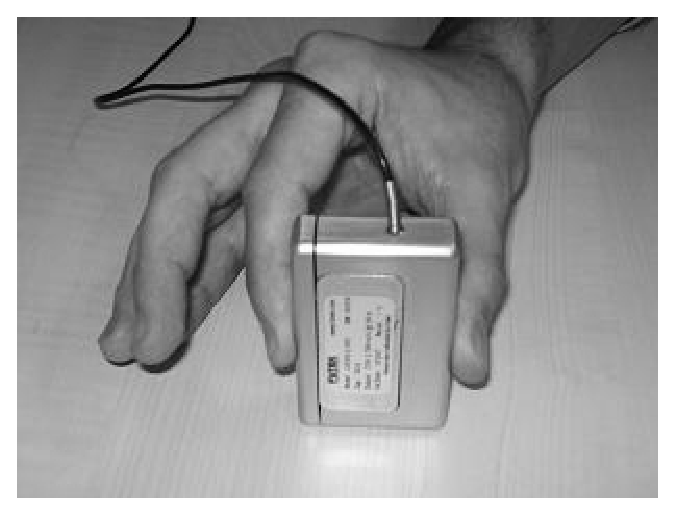
\includegraphics[height=0.16\textheight]{grip1.eps} &
%    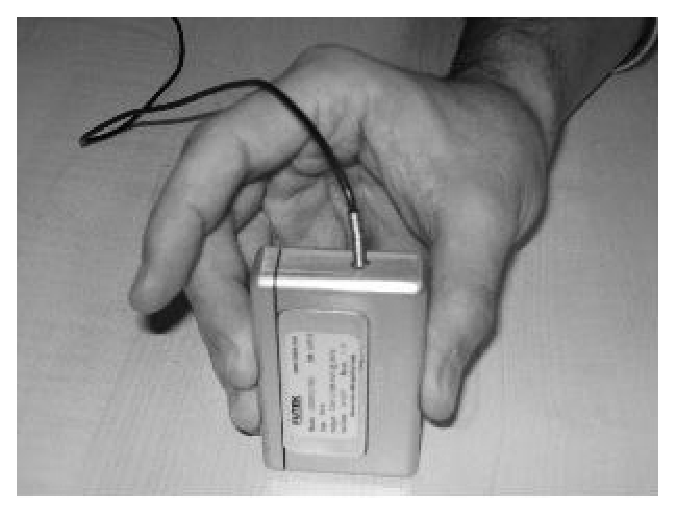
\includegraphics[height=0.16\textheight]{grip2.eps} &
%    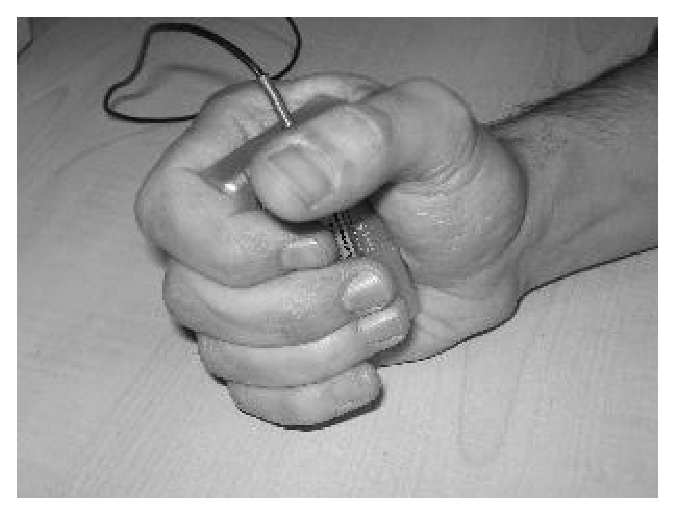
\includegraphics[height=0.16\textheight]{grip3.eps} \\
%    $(a)$ & $(b)$ & $(c)$ \\
%  \end{tabular}
%  \caption{The three different grips employed in the experiment: $(a)$
%   index precision grip; $(b)$ other fingers precision grip; $(c)$
%   power grasp.}
%  \label{fig:Grasps}
%\end{figure*}

A rest condition was sampled beforehand to define the baseline of the
EMG activity. The subject freely repeated each grasping action for
$100$'', resting for $30$'' in between grasps. The whole procedure was
repeated twice, in order to gather more data and diminish the effect
of local, statistically irrelevant, errors. Since during these
activities the subject would lie in a highly controlled position
(relaxed arm and sitting posture), this phase will
be referred to from now on as the \emph{Still-Arm phase (SA)}.

Phase $2$, actually the more interesting one for the final intent of
this study, consisted in repeating phase $1$ in a less controlled
condition: the subject was asked to grasp the force sensor while
freely moving, walking around, lifting and pronating / supinating the
arm and forearm, sitting down and standing up from a chair; this would
emulate the main movements that one is expected to do during his DLAs.
This second phase will be called \emph{Free-Arm phase (FA)}.

As a whole, each subject's experiment resulted in something more than
$1200$'' of data; at the above mentioned sampling rate of $2$KHz, this
makes it for about $2.4\times 10^6$ samples for each subject, equally
distributed in each phase.

\subsection*{Data pre-processing}

Unlike commercial EMG electrodes, such as, e.g., Otto Bock's MyoBock
electrodes \cite{ottobock}, the electrodes employed here would return
the ``raw'' EMG signal, without any low-pass filtering or Root-Mean
Square (RMS) processing. Nevertheless, it is well-known (see, again,
\cite{deluca,zecca}) that muscular activity, namely the force exerted
by a muscle, is strongly related to the RMS of the EMG signal, rather
than to the raw signal. For this reason, and also in order to aim at a
more practical, commercial implementation, we decided to evaluate the
RMS of the obtained EMG signals, electrode by electrode.

For a given mono-variate discrete time-varying signal, the RMS is
defined as the mean of the squares of the signal values, evaluated
over a certain time-window $T_{RMS}$. Roughly speaking, the RMS acts
like an envelope extraction plus a low-pass filter, whose cutoff
frequency grows smaller as the time-window grows larger (i.e., as
$T_{RMS}$ becomes higher). For this reason, high values of $T_{RMS}$
imply an ostensible delay in the resulting signal that is due to
\emph{responsiveness} of the synthesized output signal. It becomes
slower and slower as the $T_{RMS}$ value increases, since more samples
must be stored before a significant value can be evaluated.  The
choice of $T_{RMS}$ is therefore crucial in order to produce a signal
which is maximally related to the force signal, unaffected by
high-frequency noise, and with an acceptable lag. However, it must be
noted here that the EMG signal, being directly related to the muscle
\emph{activation potentials}, happens to \emph{anticipate} the muscle
movements by a few hundreds milliseconds\footnote{The
electromechanical delay (EMD) of a muscle is defined as the interval
between the onset of the electrical activity of the muscle (EMG)
indicating its activation by the neural system and the onset of the
resulting change in the mechanical variable observed. The delays
reported range from 25 to 100 ms for different muscles and tasks
\cite{Wolf1994}.}; therefore, in a practical application, a wider lag
is acceptable than one would expect. This is useful since it allows us
to increase $T_{RMS}$, if necessary.

%\begin{figure*}[!ht] \centering
%  \begin{tabular}{cc}
%    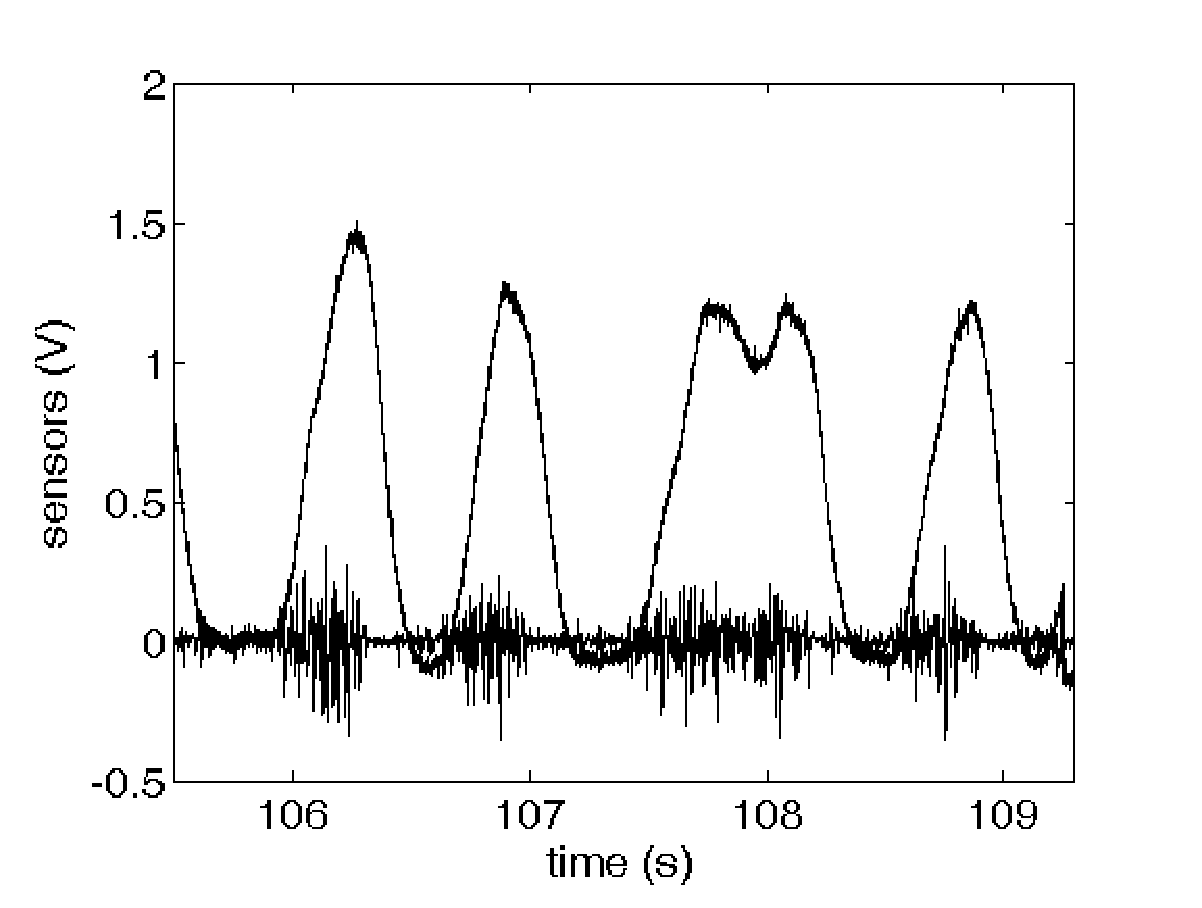
\includegraphics[width=0.45\textwidth]{force_raw.eps} &
%    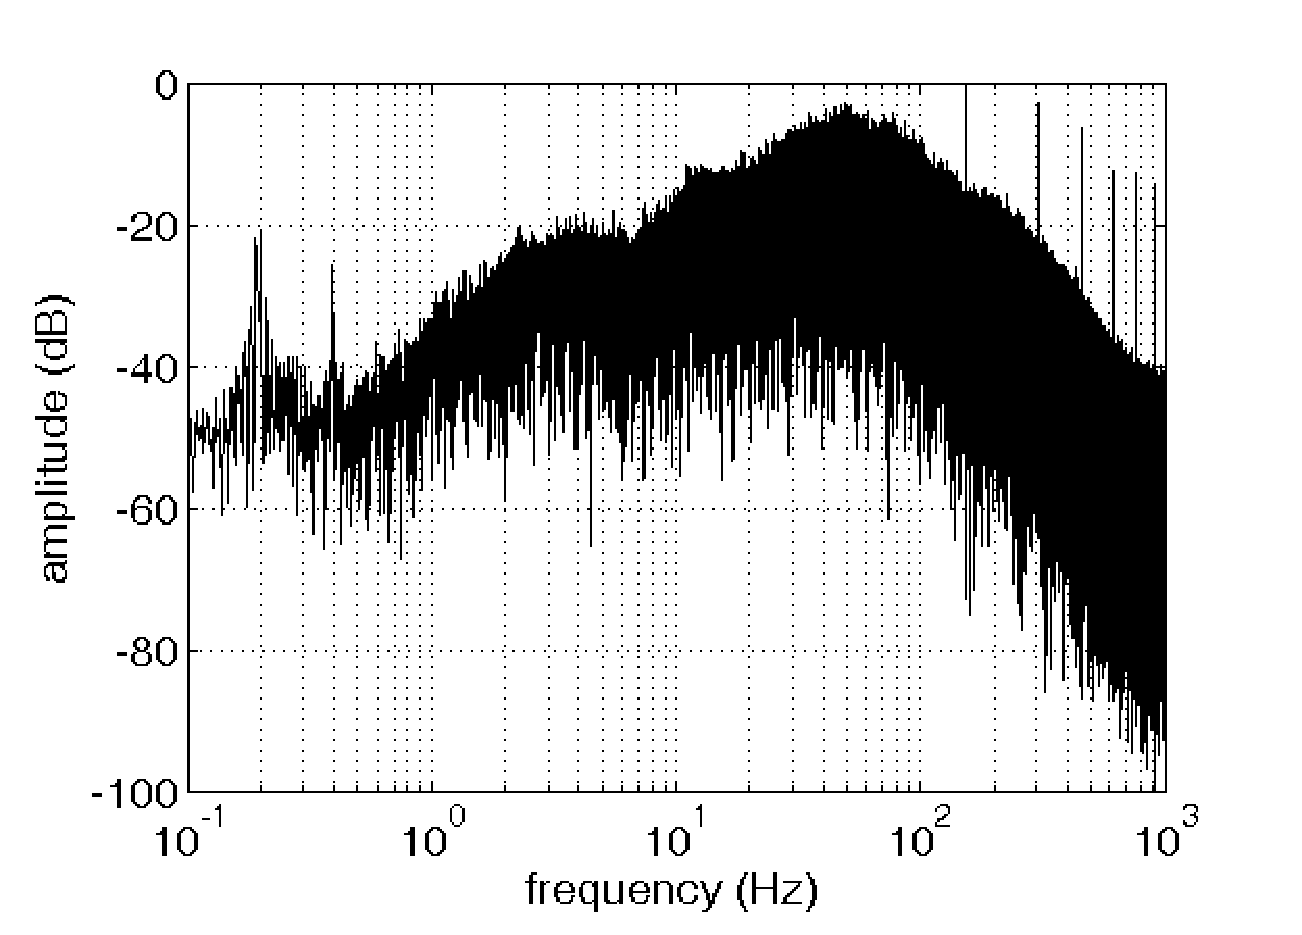
\includegraphics[width=0.45\textwidth]{spectrum_raw.eps} \\
%    $(a)$ & $(b)$ \\
%  \end{tabular}
%  \caption{$(a)$ typical raw EMG and force signals (the EMG signal
%    being the bottom, high-frequency one); $(b)$ frequency diagram of
%    the EMG signal.}
%  \label{fig:spectra}
%\end{figure*}

%\begin{figure*}[!ht] \centering
%  \begin{tabular}{ccc}
%    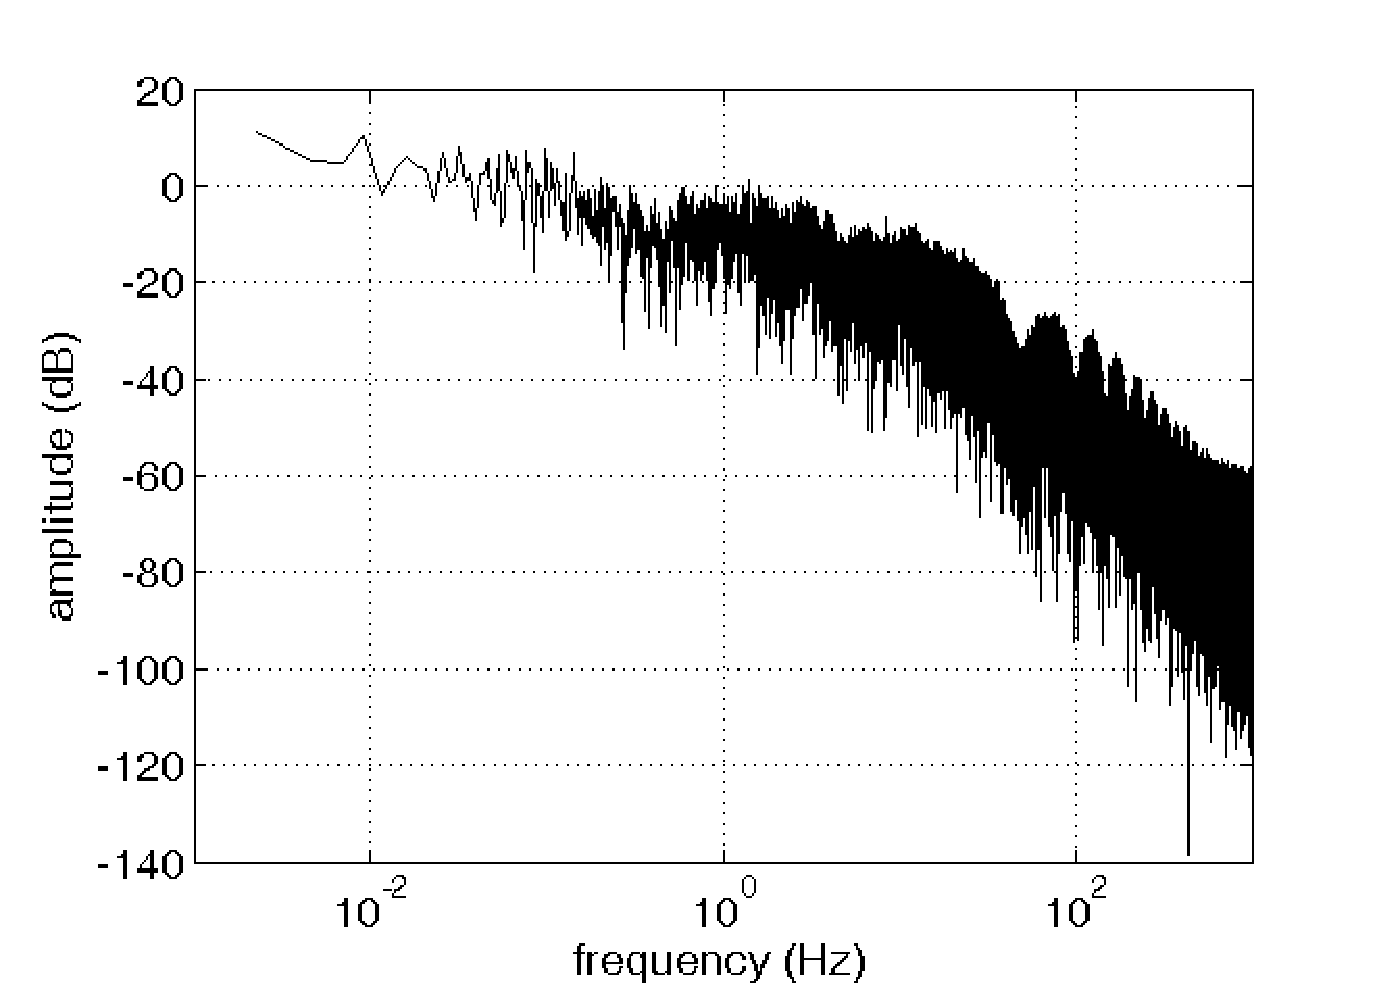
\includegraphics[width=0.3\textwidth]{spectrum_RMS0040.eps} &
%    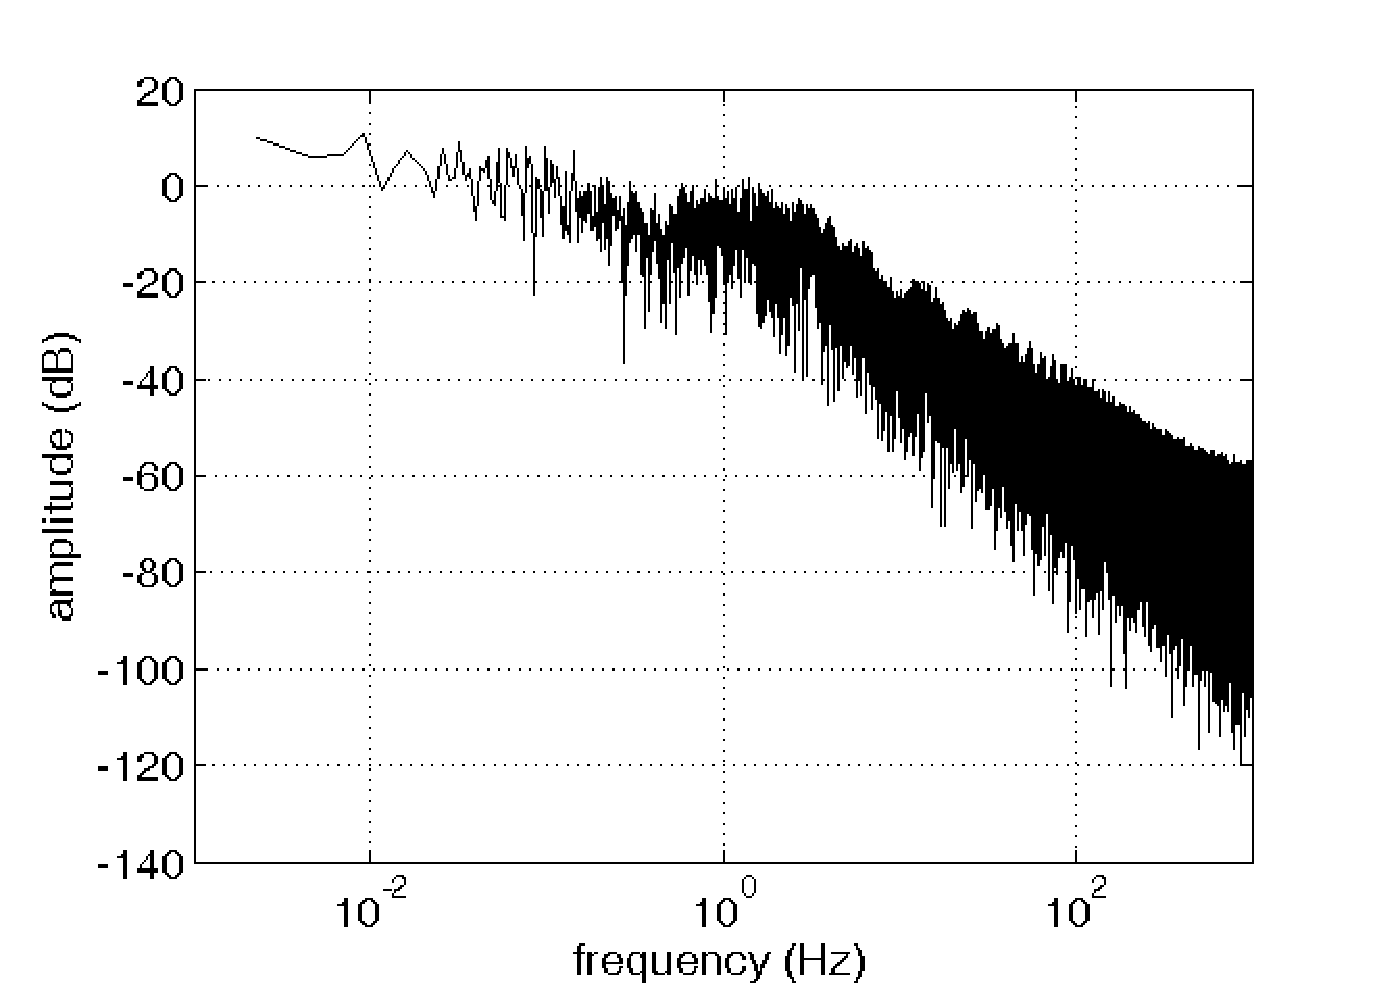
\includegraphics[width=0.3\textwidth]{spectrum_RMS0200.eps} &
%    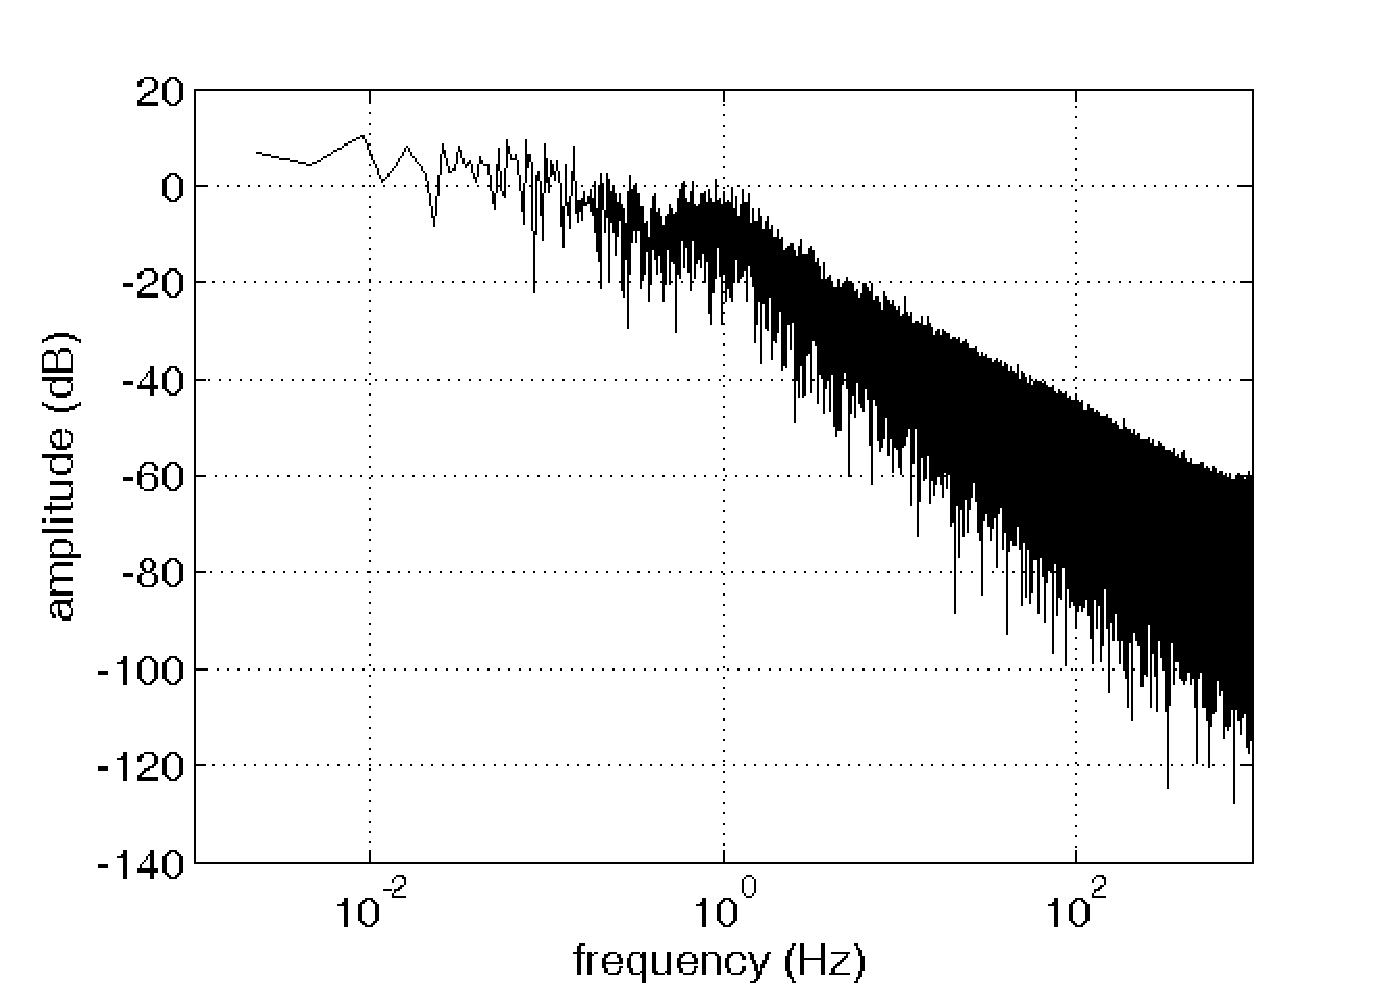
\includegraphics[width=0.3\textwidth]{spectrum_RMS1000.eps} \\
%    $(a)$ & $(b)$ & $(c)$ \\
%  \end{tabular}
%  \caption{(left to right) effects of the RMS on the bandwidth of the EMG
%    signals, for $T_{RMS} = 20, 100, 500ms$.}
%  \label{fig:RMSs}
%\end{figure*}

Unfortunately we are unaware of any systematic way of setting a good
value of $T_{RMS}$ in such a framework; the Otto Bock electrodes' one
is not mentioned either in the related technical specification
sheet. Therefore we found $T_{RMS}$ heuristically, according to some
initial experiments. See the next Section for more details. As an
example, though, consider Figures \ref{fig:spectra} and
\ref{fig:RMSs}.

Figure \ref{fig:spectra} (panel $(a)$) shows a few seconds of typical
force / EMG behaviour: it is apparent that the EMG signal (the bottom
one, with high frequencies) starts oscillating when the force signal
(the top one) starts increasing. It is also quite clear that the
amplitude of the envelope of the EMG is related to the force, as is
indicated in literature. Panel $(b)$ shows the frequency analysis of
the same EMG signal: as one can see, the meaningful bandwidth lies in
the interval known from the literature.

On the other hand, Figure \ref{fig:RMSs} shows the effect of the RMS
on the frequency components of the EMG, for three different values of
$T_{RMS}$. It is clear that the meaningful bandwidth now contains all
low-frequency components, possibly down to the constant, and is
upper-bounded by about $25$Hz (panel $(a)$, for $T_{RMS}=20ms$) to
$10$Hz (panel $(c)$, for $T_{RMS}=0.5s$). As expected, larger values
of $T_{RMS}$ correspond to a better filtering but also to a larger
delay.

This enables us to safely sub-sample the EMG signal after the RMS has
been applied. Assuming that $T_{RMS}$ is not too small, we have
subsampled both the EMG and force signal at $25$Hz, taking one sample
in $80$ of the original sequence. This has considerably reduced the
amount of data to be processed, namely to about $30.000$ samples for
each subject.

As a last data pre-processing step, we removed from the sample set
those samples for which the applied force was lower than a specific
threshold, in order to get a clearer representation of the activation
potentials. Of course, we fully retained the samples corresponding to
the baseline rest condition. This is why we preferred to record this
condition before the rest of the experiment.

\subsection*{Support Vector Machines}

According to \cite{2008.ICRA,2008.BioCyb}, where a detailed
comparative analysis among three different machine learning methods
was carried out, we chose to employ Support Vector Machines (SVMs) to
solve our problem. For an explanation of how SVMs work in the context
of EMG signals, please refer to those papers; for a comprehensive
tutorial on SVMs in the more general framework of
\emph{classification} and \emph{regression}, refer to
\cite{Burges98,SmolaTut2004}.

Suffice it here to say that SVMs are a statistical learning method
able to build an approximated map between an input space and a label
(classification) or a real value (regression). Classification is here
used to classify the type of grasp according to the EMG signal,
whereas regression is used to understand how much force the subject is
exerting, independently from the grasp type; the input space is then
$\RR^7$, one coordinate for each EMG electrode; the labels are four
integer numbers, one for each grasp type; and the real value is
exactly the force value read off the force sensor.

SVMs are a \emph{supervised learning} approach, meaning that they must
first be \emph{trained} on an EMG dataset for which labels and force
values are known, in order to build the required input/output map; and
then they can be used to \emph{predict} the values of new EMG samples,
using the map. Notice that we work in real-time, that is, our machines
associate a grasp type and a force value to an EMG value \emph{at each
instant of time}. This approach enables us to detect a grasp type
\emph{almost at the onset of the grasping movement}\footnote{the
precise onset of the movement would correspond to those samples which
were removed since they were associated to too low a force value.},
differently from what happens in other approaches (e.g.,
\cite{smagt,Sebelius2005}) in which all values of the input signal over a
further time-window are employed as the input space, in order to let
the system understand better the final grasp type.

Lastly, SVMs are known to suffer from heavy computational needs when
it comes to training on large datasets: training on these datasets
would have then been prohibitive. Moreover, the general aim of our
research is to build an on-line system, able to predict in a very
short amount of time; and in on-line learning the flow of training
data is potentially endless. So we need a way of checking whether the
EMG samples used for training are useful, rejecting the ones deemed
useless. This is supposed to eventually keep the training set bounded,
and dramatically reduce the training set size in this particular
experiment, where the training time is rather small if compared to a
real-life setting. We employ \emph{uniformisation}
\cite{2008.ICRA,2008.BioCyb} to do this: given a \emph{minimum
distance} $d > 0$, we reject those samples which are too close to each
other, with the underlying assumption that the maps we are trying to
build are smooth enough to allow such a simplification. More in
detail, the samples in a training batch are considered one by one in
chronological order, as it would happen in an on-line setting; each
new sample is then added to the training set if, and only if, its
distance from all training samples retained so far is at least
$d$.

%\begin{figure*}[!ht] \centering
%  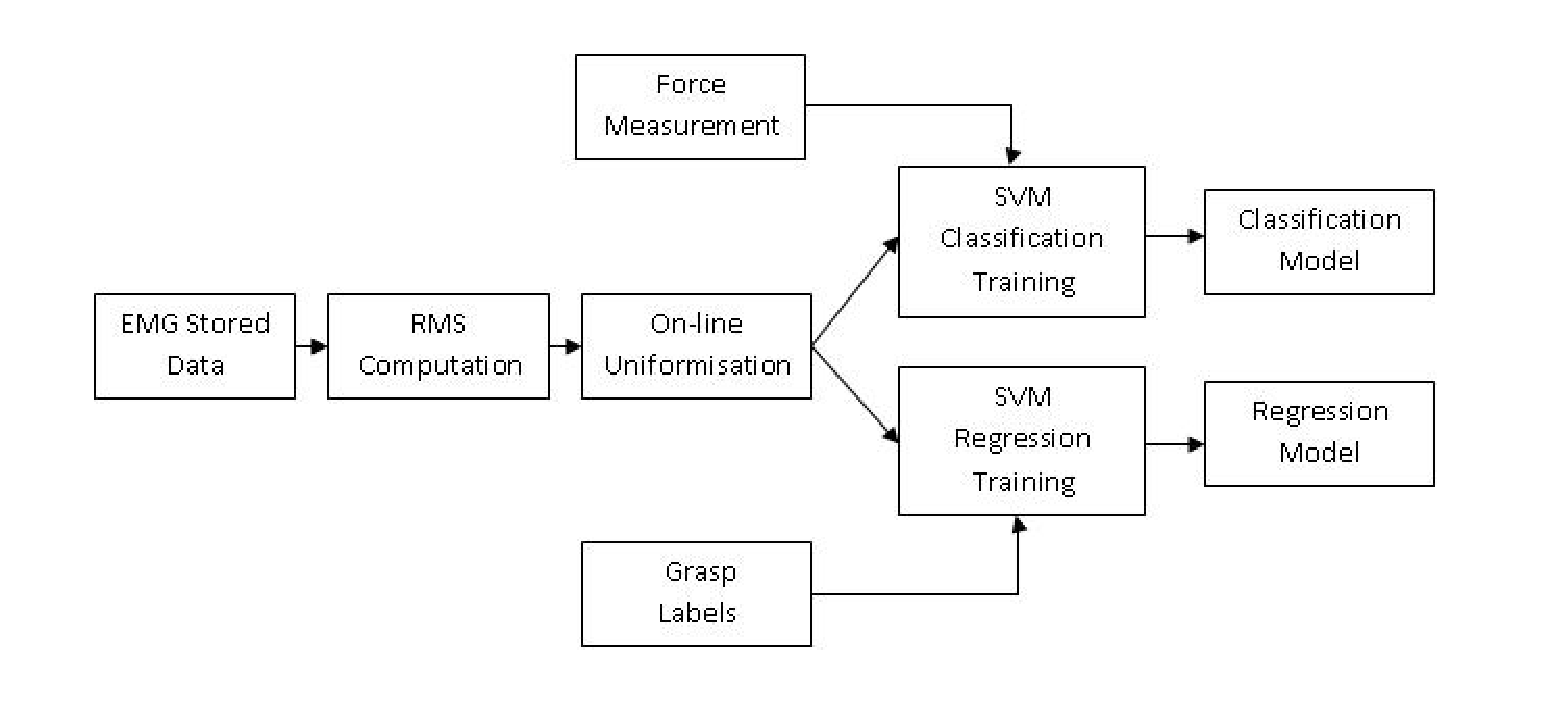
\includegraphics[width=0.75\textwidth]{Schema.eps} \\
%  \caption{Graphical representation of the system employed to solve our problem.}
%  \label{fig:Algorithm}
%\end{figure*}

Figure \ref{fig:Algorithm} graphically depicts the structure of our
system, finally producing the classification and regression models,
which will be then used for the prediction. Notice that there can
actually be two different RMS windows, one for classification and one
for regression.

\section*{Results and Discussion}
\label{sec:exp}

This Section is a detailed account of the experimental results. It is
worth to repeat once again what the main questions are, in the light
of the long-term aim of this research. It is already known that SVMs
applied to this problem, \emph{for one healthy subject} and \emph{in
highly controlled conditions} can solve it. Now,

\begin{enumerate}

  \item can they be successfully applied to \emph{any} subject?

  \item will they work in non-controlled conditions?

\end{enumerate}

The first question is tantamount to asking whether a uniformly good
performance can be obtained for each subject; the second question is
equivalent, in our framework, to asking whether the performance is
comparable between the SA and FA phases.

\subsection*{Per-Subject Analysis}

For each of the $10$ subjects, and for each phase (SA and FA) we
hereby present a performance result both for classification and
regression. For classification, the performance index is, as is
customary, the percentage of overall correctly guessed labels. For
regression, the performance index is the correlation coefficient
evaluated between the predicted force signal and the real one. The
choice of the correlation coefficient, as opposed to the more standard
Mean-Square Error, is suggested by a practical consideration: when
driving a prosthesis, or even a non-prosthetic mechanical hand, we are
not interested in the absolute force values desired by the
user/subject, since mechanical hands usually cannot apply as much
force as human hands do, for obvious safety reasons\footnote{or, e.g.,
in teleoperation scenarios, they could be able to apply \emph{much
more} force than a human hand can.}. We are rather concerned about
getting a signal which is \emph{strongly correlated} with the
user/subject's will.

As is standard in machine learning, each data set was split in $5$
folds and cross-validation was performed on it; this makes the
evaluation robust against the problem of over-fitting. In all our
tests, the training sets were uniformised using a minimum distance
threshold $d$, but no testing sets were uniformised, of course. We
employed a well-known freely available SVM package, \emph{libsvm}
v2.83 \cite{ChangL01}, in the Matlab wrapped flavour, with a Gaussian
kernel. This particular kind of SVM requires setting two
\emph{hyperparameters}, called $\gamma$ and $C$, which were found by
grid search using the aforementioned performance indexes.

With respect to the previous Section, after an initial round of
experiments the values of $T_{RMS}$ and $d$ were set to:

\begin{itemize}

  \item $T_{RMS}=0.5s$ for classification, and $T_{RMS}=0.1s$ for regression;

  \item $d=0.02$ for the SA phase, and $d=0.032$ for the FA phase.

\end{itemize}

Classification proved to be more sensitive to high-frequency noise
than regression, and therefore we set a larger value of $T_{RMS}$ for
it; it is expected, anyway, that the low responsiveness of the RMS
signal computed on a $500ms$ window would be compensated at least
partially by the anticipatory nature of the EMG signal. This should
not, then, hinder the performance of the system in a practical
setting. As far as the values of $d$ are concerned: we chose the above
mentioned values in order to get not more than one thousand training
samples for subject $1$.  This proved to be a sensible choice, as we
will see. Notice that (see \cite{2008.BioCyb}) the performance of such
systems changes linearly as $d$ changes, whereas the training set size
varies polynomially; thus, it is always possible to find a
polynomially smaller training set, if needed, which will degrade the
performance only linearly. This really means that the initial choice
of $d$ is not that important. See the end of this Section for a deeper
analysis.

Figure \ref{fig:results} shows the main results obtained by the SVMs.

%\begin{figure*}[!ht] \centering
%  \begin{tabular}{cc}
%    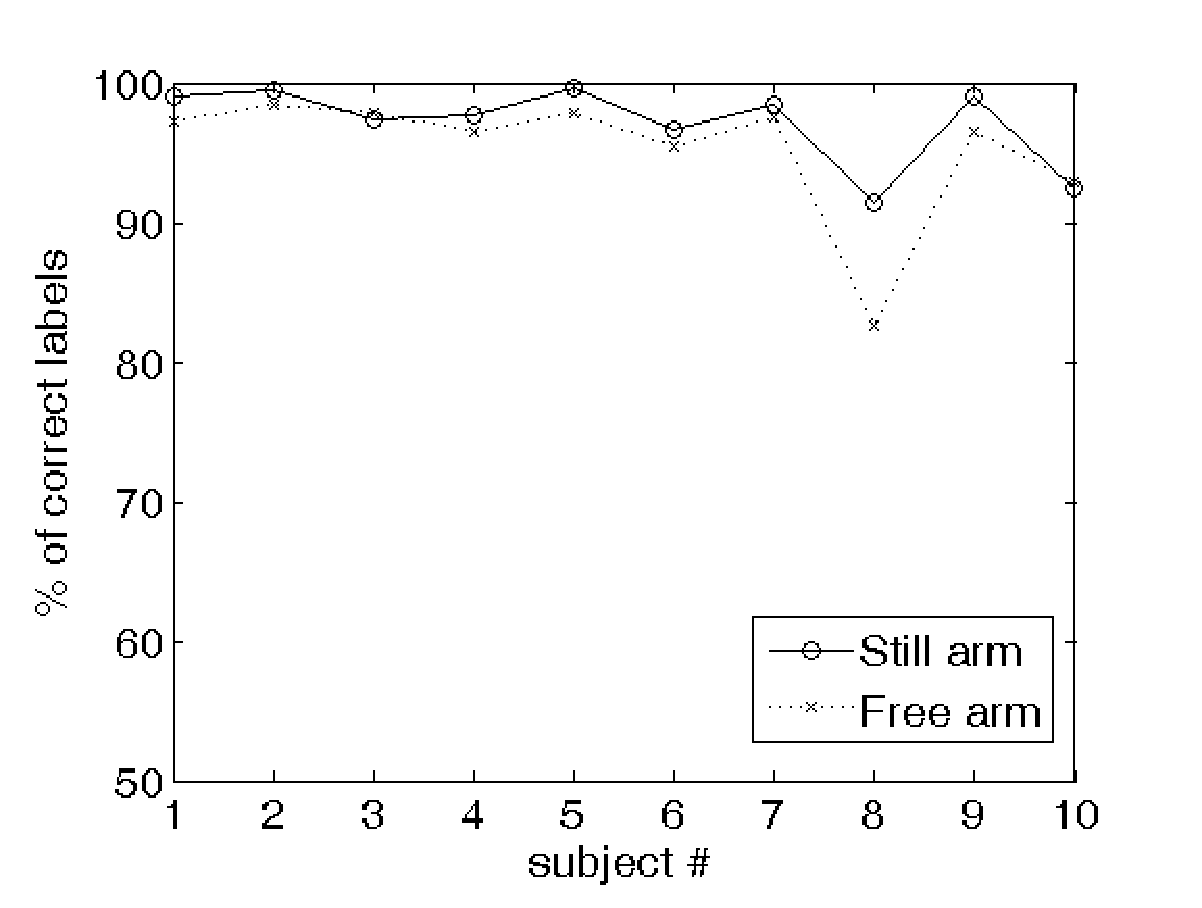
\includegraphics[width=0.45\textwidth]{perfClass.eps} &
%    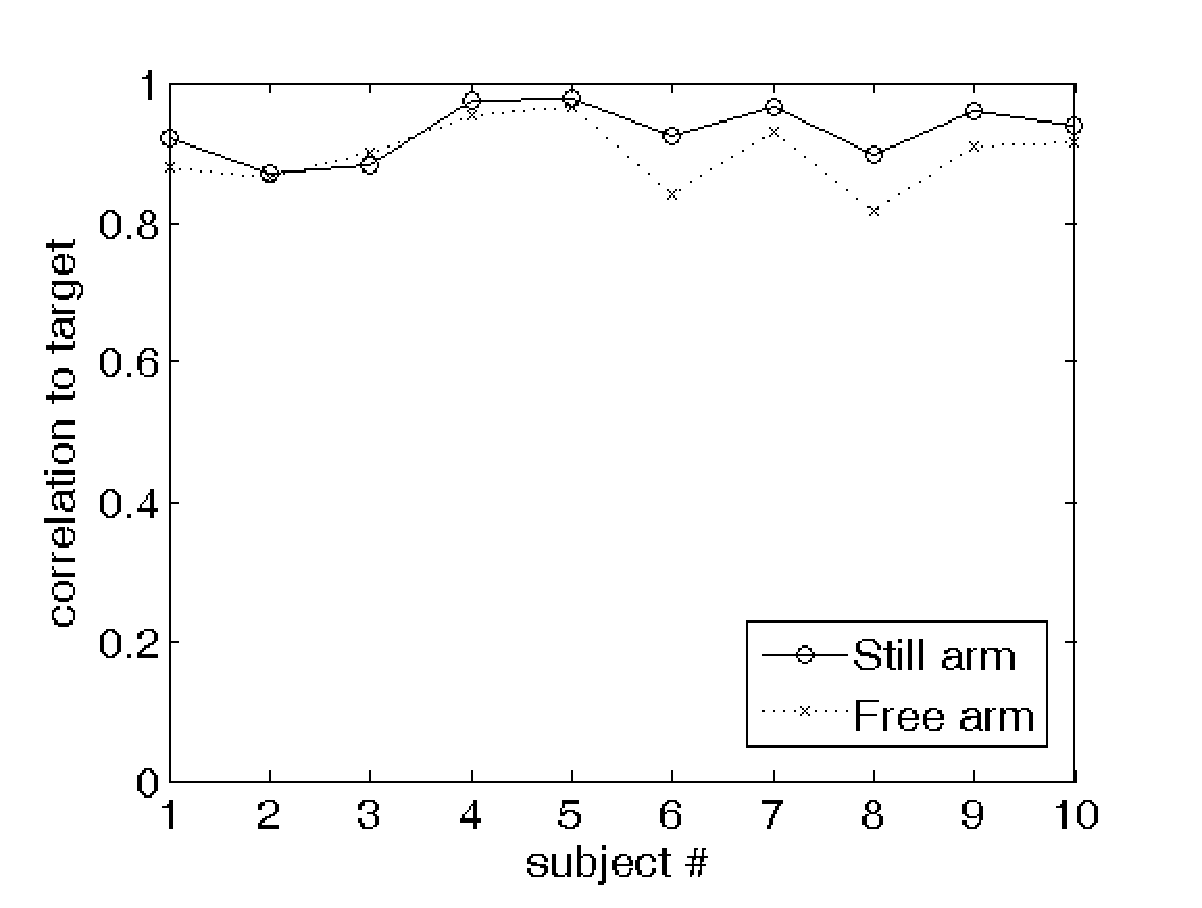
\includegraphics[width=0.45\textwidth]{perfRegr.eps} \\
%    $(a)$ & $(b)$ \\
%  \end{tabular}
%  \caption{classification $(a)$ and regression $(b)$ results obtained
%    by the system, on both phases of the experiment (FA and SA) and
%    for each subject.}
%  \label{fig:results}
%\end{figure*}

Consider the Figure, panel $(a)$, showing the classification
performance. It is clear that the system attains an excellent accuracy
overall, namely $97.14\% \pm 2.89\%$ on average in the SA phase, and
$95.28\% \pm 4.73\%$ in the FA phase. Moreover, the performance is
consistent by subject and by phase, meaning that $(a)$ hard subjects
in the SA phase are hard as well in the FA phase and viceversa, and
$(b)$ the FA phase is always harder than the SA phase. Less controlled
conditions make the problem harder, as one would expect, but the
performance remains very good to excellent.

Consider now panel $(b)$ of the same Figure, showing the regression
performance: again the results are excellent, being $0.93
\pm 0.04$ for the SA phase and $0.90 \pm 0.05$ for the FA
phase. Again, consistency by subject and by phase appears. Remarkably,
not all subjects which are slightly harder for regression (namely,
$1,2,3,6,8$) happen to be hard for classification; in particular, only
subject $8$ is definitely hard \emph{both} for classification and
regression, while, e.g., subject $6$ is hard for regression but not
that hard for classification.

As an example of what the system can really do, Figure
\ref{fig:examples} shows the real and guessed force values for a
typical subject, namely number $6$, FA phase. As one can visually
check, the guessed force values are highly correlated to the real
values.

%\begin{figure*}[!ht] \centering
%  \begin{tabular}{cc}
%    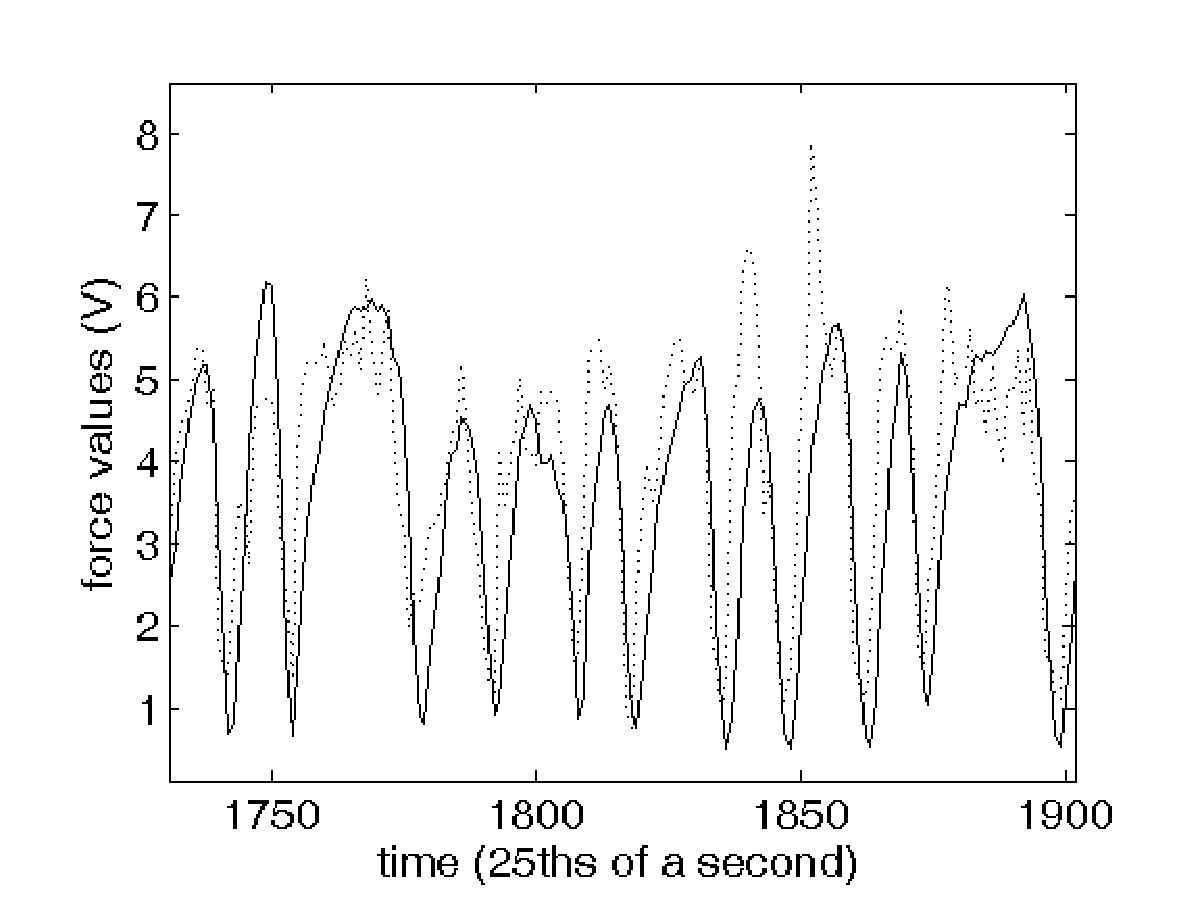
\includegraphics[width=0.45\textwidth]{example_6_one.eps} &
%    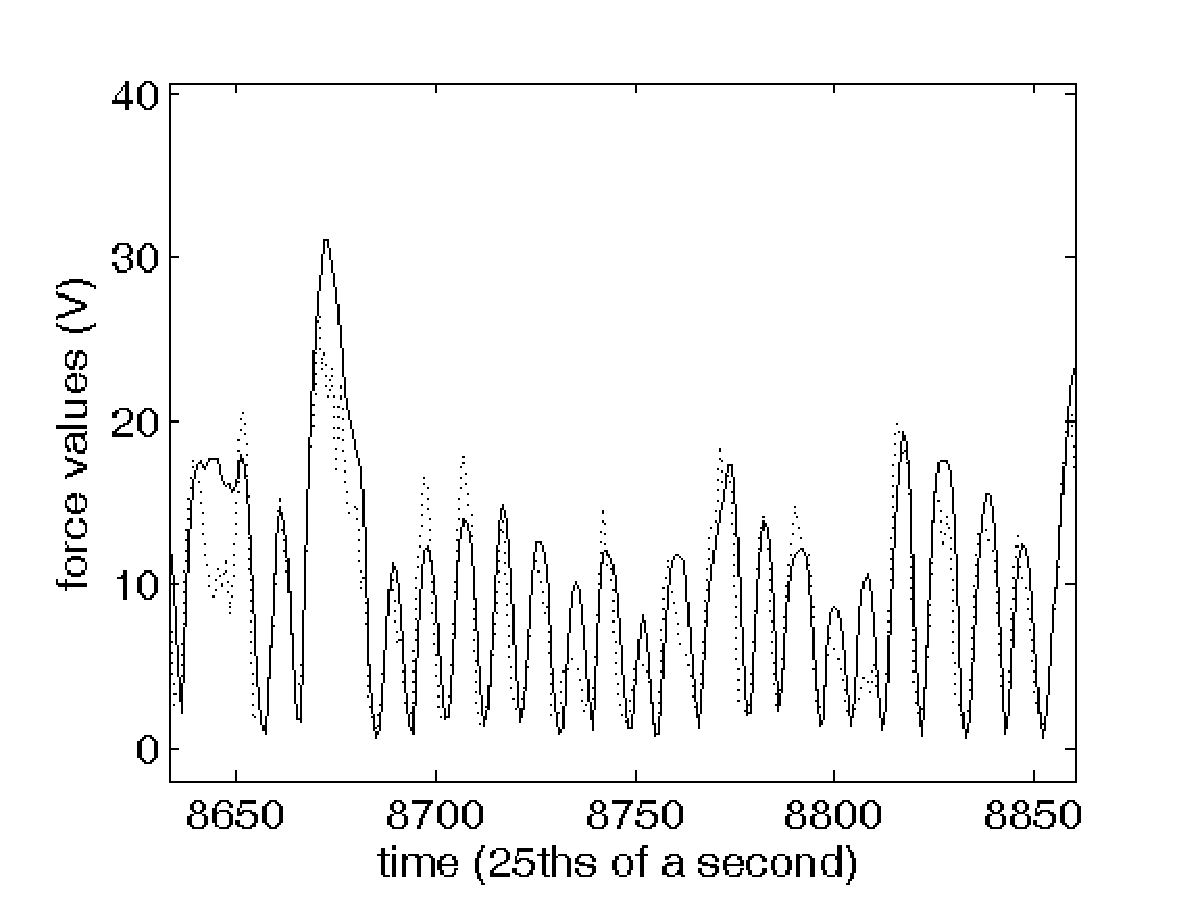
\includegraphics[width=0.45\textwidth]{example_6_two.eps} \\
%    $(a)$ & $(b)$ \\
%  \end{tabular}
%  \caption{comparing true (continuous line) and guessed (dotted line) force values for regression of a
%    typical subject (number $6$, FA phase).}
%  \label{fig:examples}
%\end{figure*}

Since we are doing multi-subject per-subject analysis here, an
interesting point is that of checking whether there are any
regularities among them, from the point of view of machine
learning. For instance, knowing that a hyperparameter takes mostly a
certain value would enable us to employ a narrower and/or quicker grid
search with new, upcoming subjects. Table \ref{tab:hyp} shows the
average values of (the logarithms of) $\gamma$ and $C$ and for the
optimal models obtained via cross-validation, as described at the
beginning of this Section.

The grid search ranges were $0$-$3$ for $log_{10}(C)$ and
$-1.85$-$0.16$ for $log_{10}(\gamma)$ (these are standard values in
literature). In view of this, we see that the average value of
$log_{10}(C)$ is around $1.5$, but its standard deviation is too wide
to allow narrowing the grid search, at least in the case of
classification. The standard deviation is smaller for regression than
for classification in both cases, which seems to indicate that
regression as a problem is more stable with respect to the
hyperparameters. In this case one can foresee a faster way of finding
the optimal hyperparameters, for example by employing a minimisation
procedure rather than grid search.

All in all, the answers to the two questions we posed at the beginning
of the Section are positive. Results are consistent and excellent for
each subject, and both for the SA and FA phases, with a special
emphasis on the latter one. Of course, one more interesting question
is: is the FA phase really indicative of what a patient might do in
her/his DLAs? Since we are claiming that the FA phase represent
something inherently more complex than the SA phase, we should be able
to see that FA-models (trained in non-controlled conditions) are to
some extent able to predict the outcomes in the SA (controlled)
conditions; of course, we expect a large amount of data to overlap, so
that the other way round would be true, too, but to a lesser
extent. Notice, by the way, that the problems of electrode
displacement and inter-arm differences are not present here, since the
electrodes were not moved between the two phases, and the experiments
are done on the same subject.

The answer is found via a kind of cross-analysis: for each subject,
and for either problem, classification and regression, we can train a
machine on the data gathered during the FA phase and then test on the
data gathered during the SA phase. Figure \ref{fig:2on1} shows the
results of testing FA-models on SA data, and viceversa.

%\begin{figure*}[!ht] \centering
%  \begin{tabular}{cc}
%    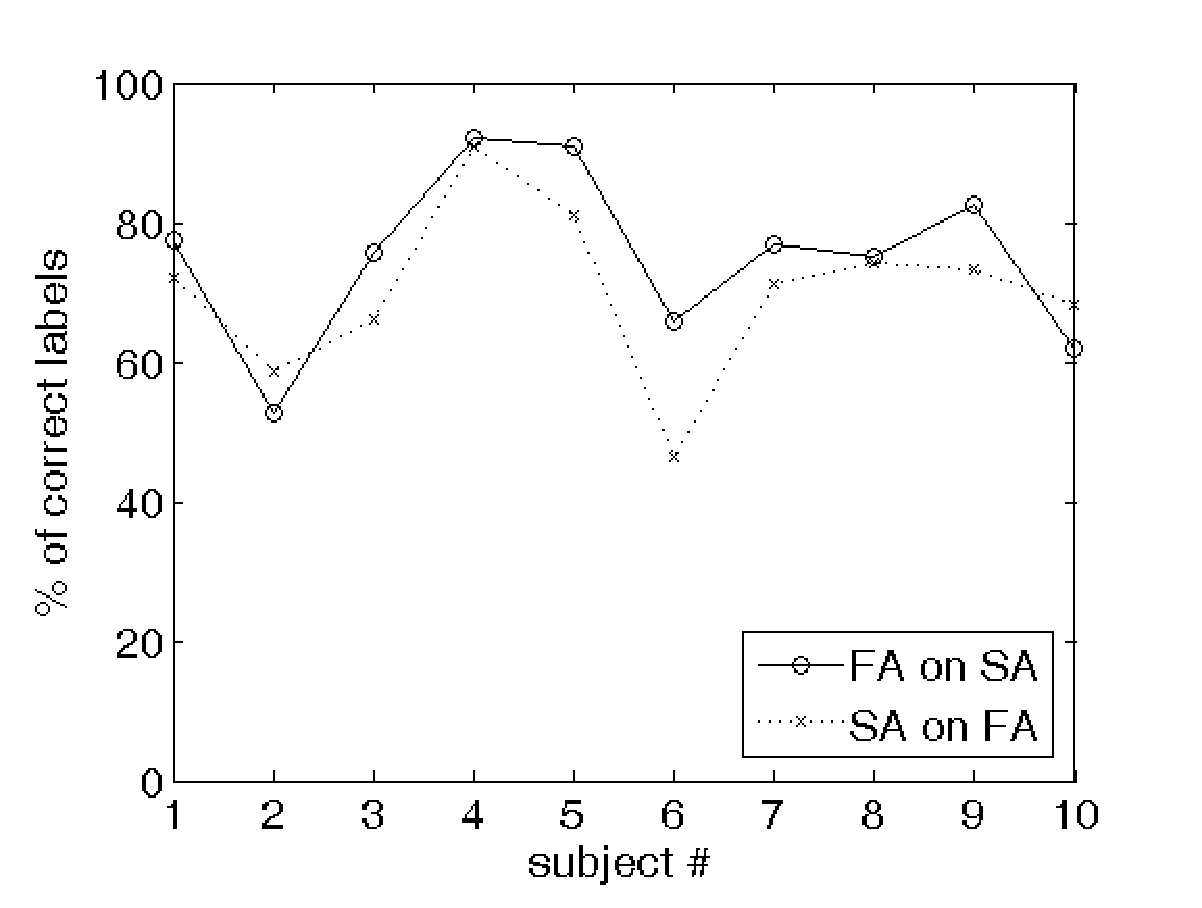
\includegraphics[width=0.45\textwidth]{2on1_class.eps} &
%    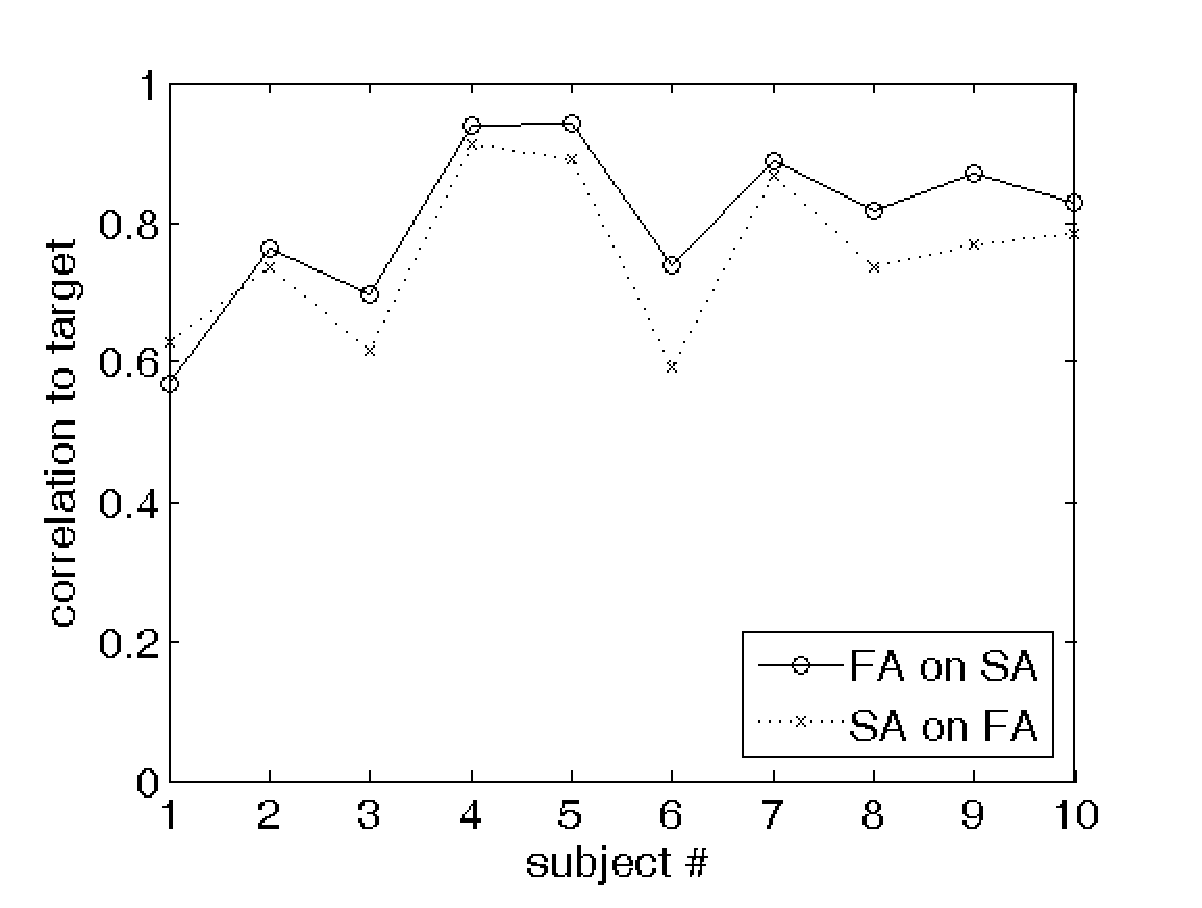
\includegraphics[width=0.45\textwidth]{2on1_regr.eps} \\
%    $(a)$ & $(b)$ \\
%  \end{tabular}
%  \caption{classification $(a)$ and regression $(b)$ results obtained
%    testing on SA-data models trained on FA, and vice-versa.}
%  \label{fig:2on1}
%\end{figure*}

First of all, both ways of testing attain good results (although, of
course, not comparable with those of the plain per-subject analysis,
compare with Figure \ref{fig:results}): testing FA-models on SA data
gives a performance of $72.11\% \pm 12.34\%$ for classification and
$0.81 \pm 0.12$ for regression; whereas testing SA-models on FA data
gives $70.17\% \pm 11.99\%$ in classification and $0.75 \pm 0.12$ in
regression. This indicates a prevalence of the former models over the
latter ones. Moreover, by considering the aforementioned Figure, it is
apparent that, almost consistently, the result obtained by FA-models
on SA data is superior with respect to the others. This indicates
that, actually, models trained on FA data ``know something more''; we
claim that this added value is given by the freedom of movement
granted to the subjects during this phase of the experiment. Together
with the fact that we are employing uniformisation, a strategy which
limits the number of samples in training sets, this lets us also claim
that, in a real setting, we could have more and more data be gathered
off ``real'' DLAs, and more and more complex models be incrementally
trained in order to adapt to a wider and wider set of actions and
situations.

Lastly, it is interesting to consider whether the still unsatisfactory
results we have can be made better, in the perspective of having, in
real life, much more data and harder problems at hand. Let us consider
the worst result of the per-subject analysis, that is, subject $8$ in
the FA phase, as far as classification is concerned. The result
attained by this subject is $82.59\%$. The most likely cause of this
low performance is that too many useful samples are missing from the
training set, that is, the minimum distace threshold $d$ was set at
too high a value. In order to test this hypothesis, and to confirm the
experimental results of
\cite{2008.BioCyb} as we said at the beginning of this Section, we
let $d$ linearly range around the pre-set value of $0.032$ and check
$(a)$ the size of the resulting training set and $(b)$ the performance
obtained by the system. Figure \ref{fig:subj8} shows the result of
this test.

%\begin{figure*}[!ht] \centering
%  \begin{tabular}{c}
%    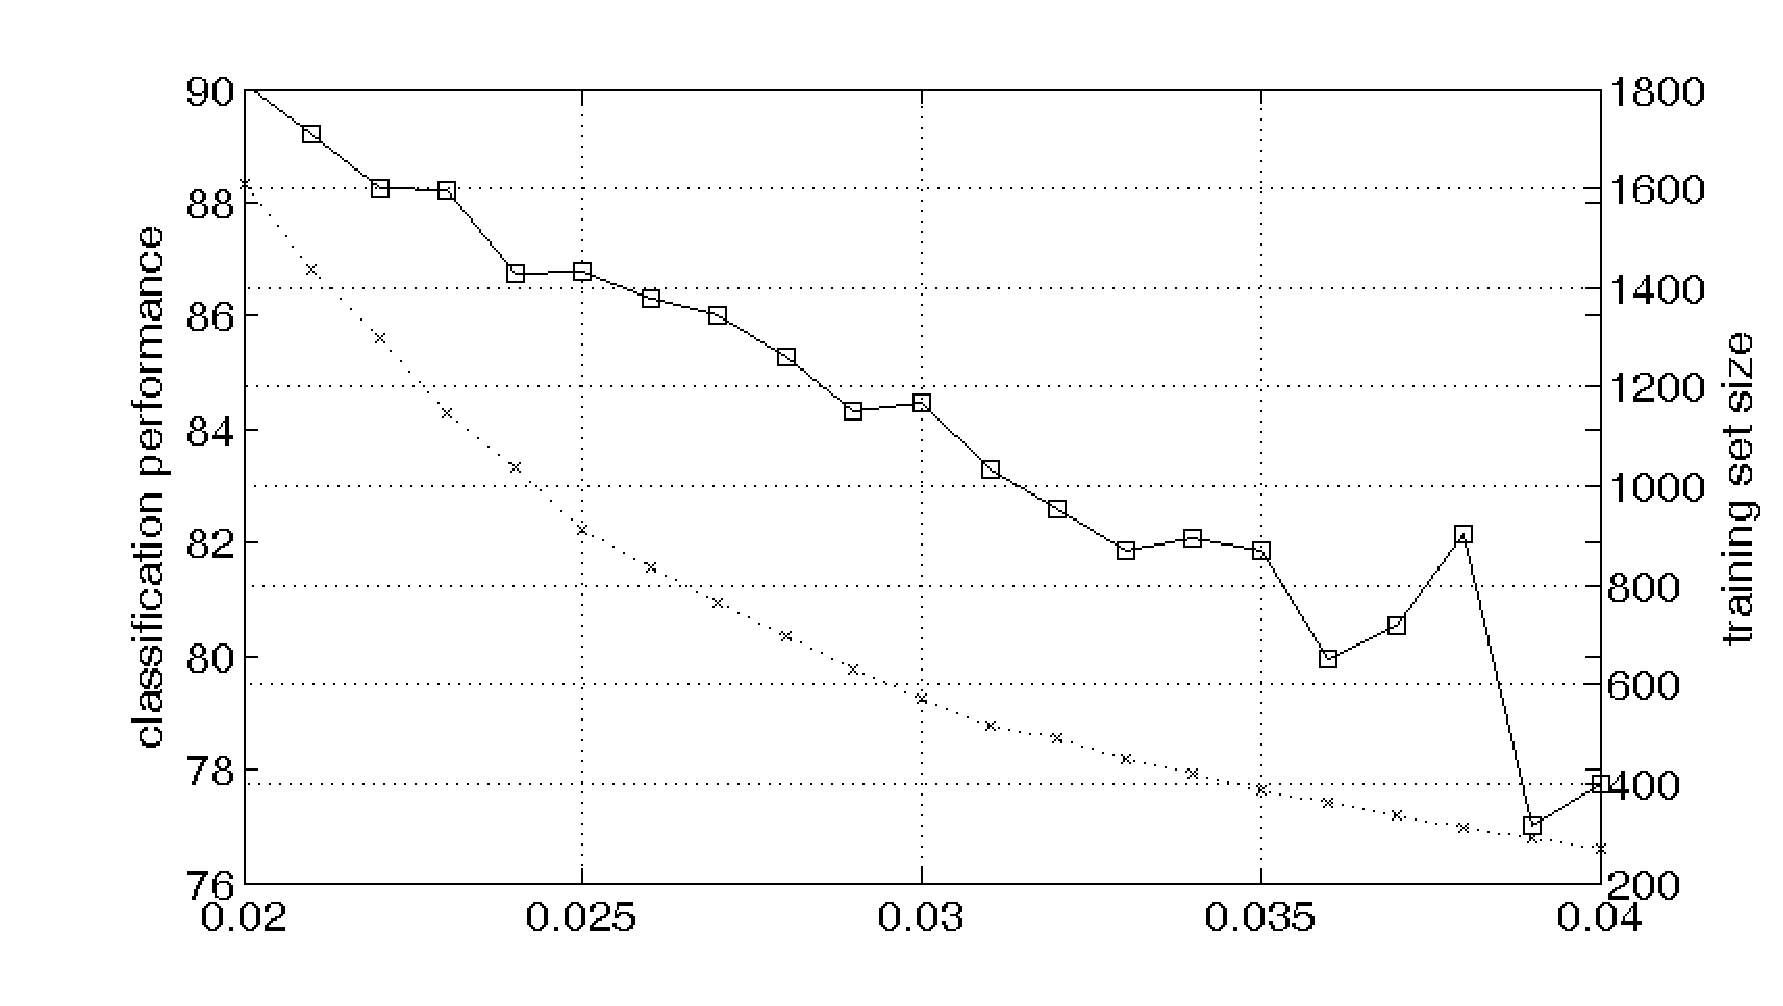
\includegraphics[width=0.6\textwidth]{subj8.eps} \\
%  \end{tabular}
%  \caption{size of the training set (dotted line) and classification
%    performance (continuous line), of subject $8$ in the FA phase, as
%    $d$ changes.}
%  \label{fig:subj8}
%\end{figure*}

The Figure confirms that the training set size has a decreasing
polynomial trend, while the performance changes linearly. In
particular, for $d=0.032$ the previously shown performance appears,
whereas if a larger performance is required, one can increase the
number of samples in the training set, or, which is equivalent, reduce
the agnitude of $d$. For instance, to get an accuracy of about $90\%$
$d$ must be set at $0.2$ ending up in a training set with some $1600$
samples.

\subsection*{Cross-Subject Analysis}

We now turn our attention to cross-subject analysis, that is, how
accurate a model trained on a subject is, if tested on data gathered
from another subject. This problem is interesting in the sense that it
can shed light on common model features, hopefully paving the way for
building a pre-trained ``universal'' model, which could be shipped
along with the mechanical hand or prosthesis, and dramatically reduce
the human subject's training time.

Recall that in this experiment, for all subjects, the EMG electrodes
were carefully positioned on the forearm according to an anatomical
guideline, meaning that noise due to inter-arm differences should be
to some extent avoided. We can therefore check how well each model
performs on each subject by building a \emph{cross-subject performance
matrix} $A$, for both classification and regression, and for both phases,
in which $A_{ij}$ is the performance index attained by a model trained
on data gathered from subject $i$ while predicting data gathered from
subject $j$. Figure \ref{fig:cross} shows the four matrices.

%\begin{figure*}[!ht] \centering
%  \begin{tabular}{cc}
%    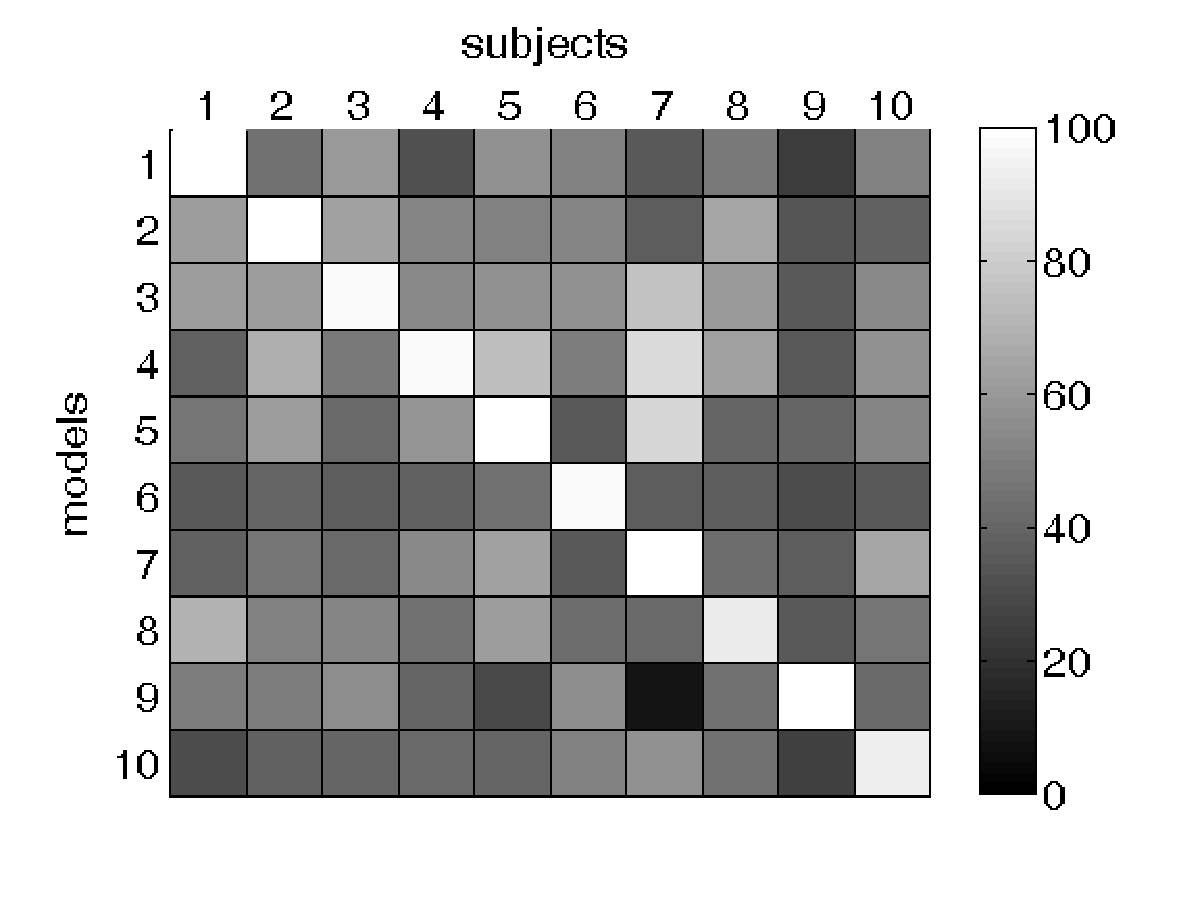
\includegraphics[width=0.45\textwidth]{crossClass1.eps} & 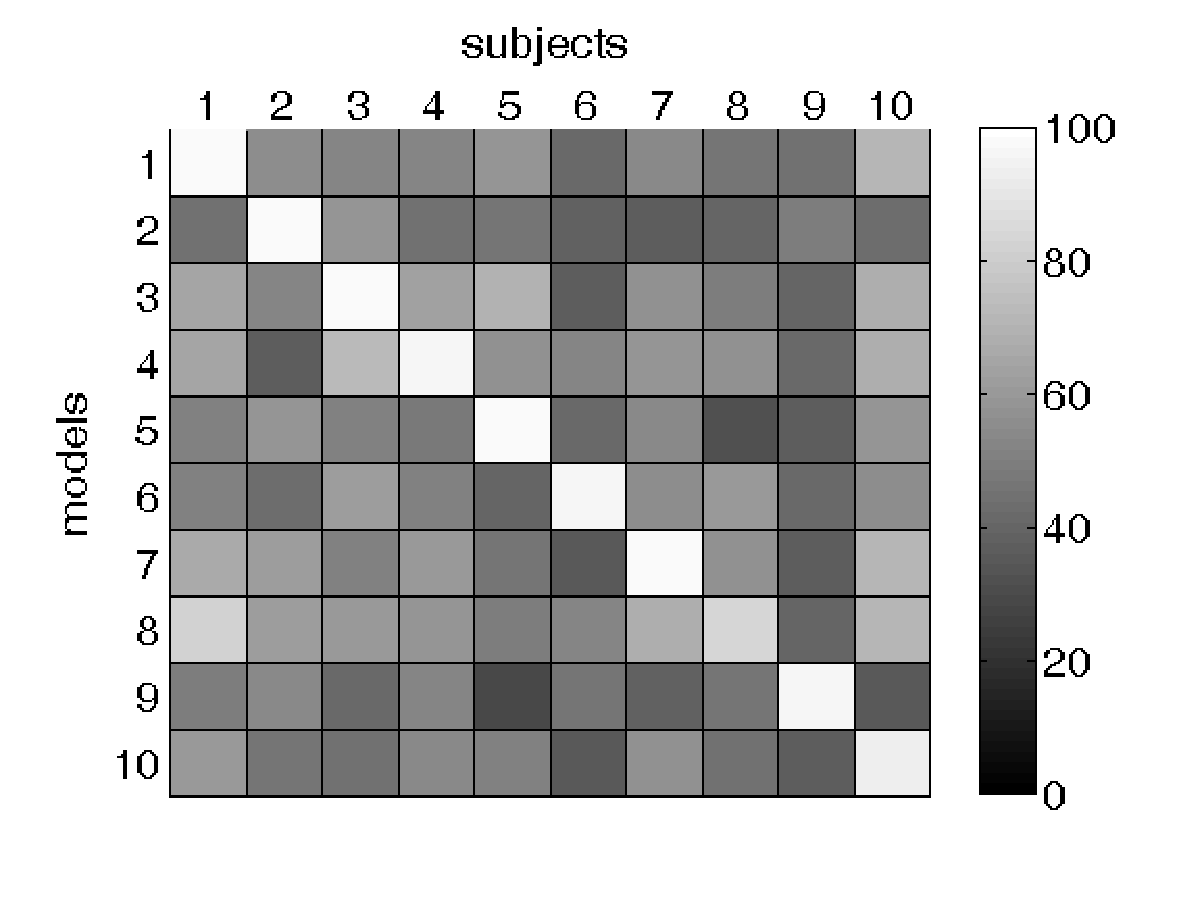
\includegraphics[width=0.45\textwidth]{crossClass2.eps} \\
%    $51.69\% \pm 19.27\%$ & $54.04\% \pm 16.42\%$ \\
%    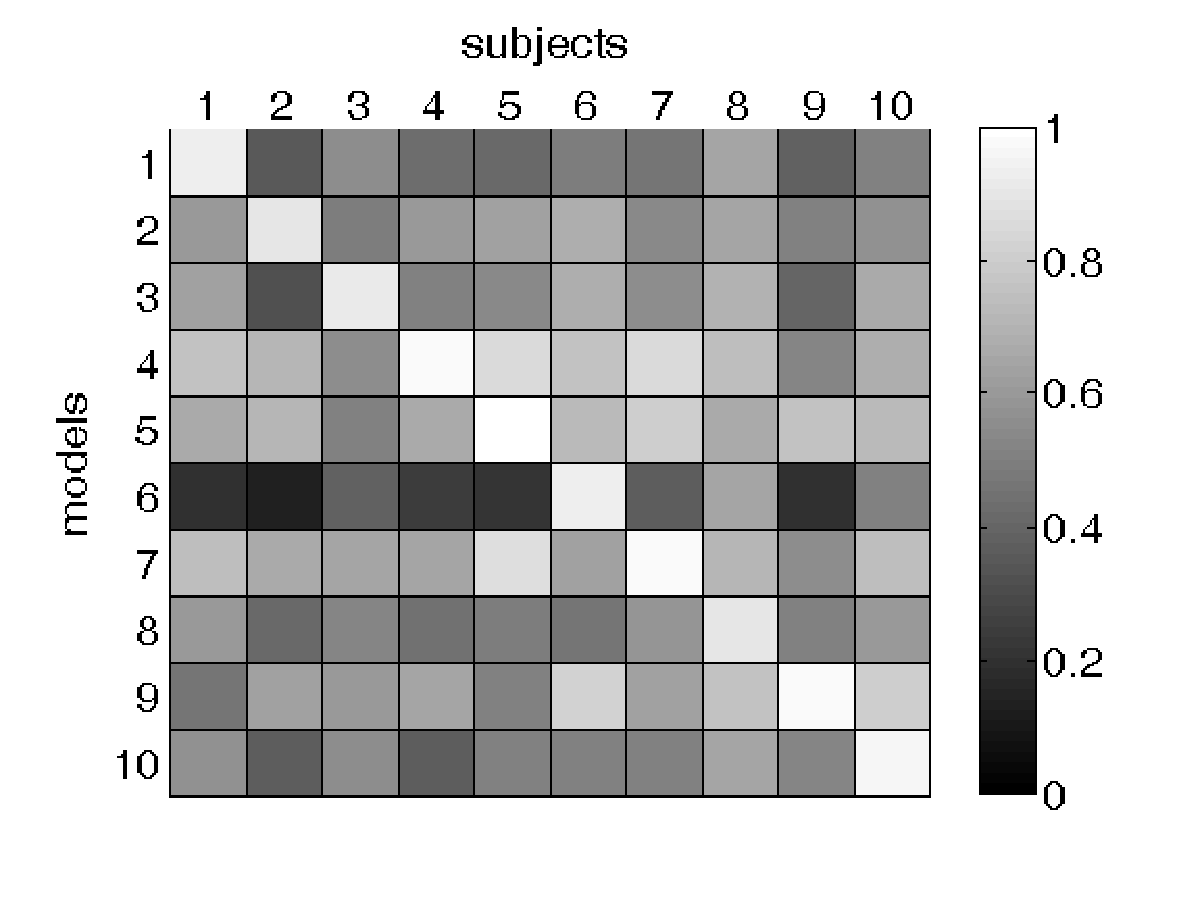
\includegraphics[width=0.45\textwidth]{crossRegr1.eps} & 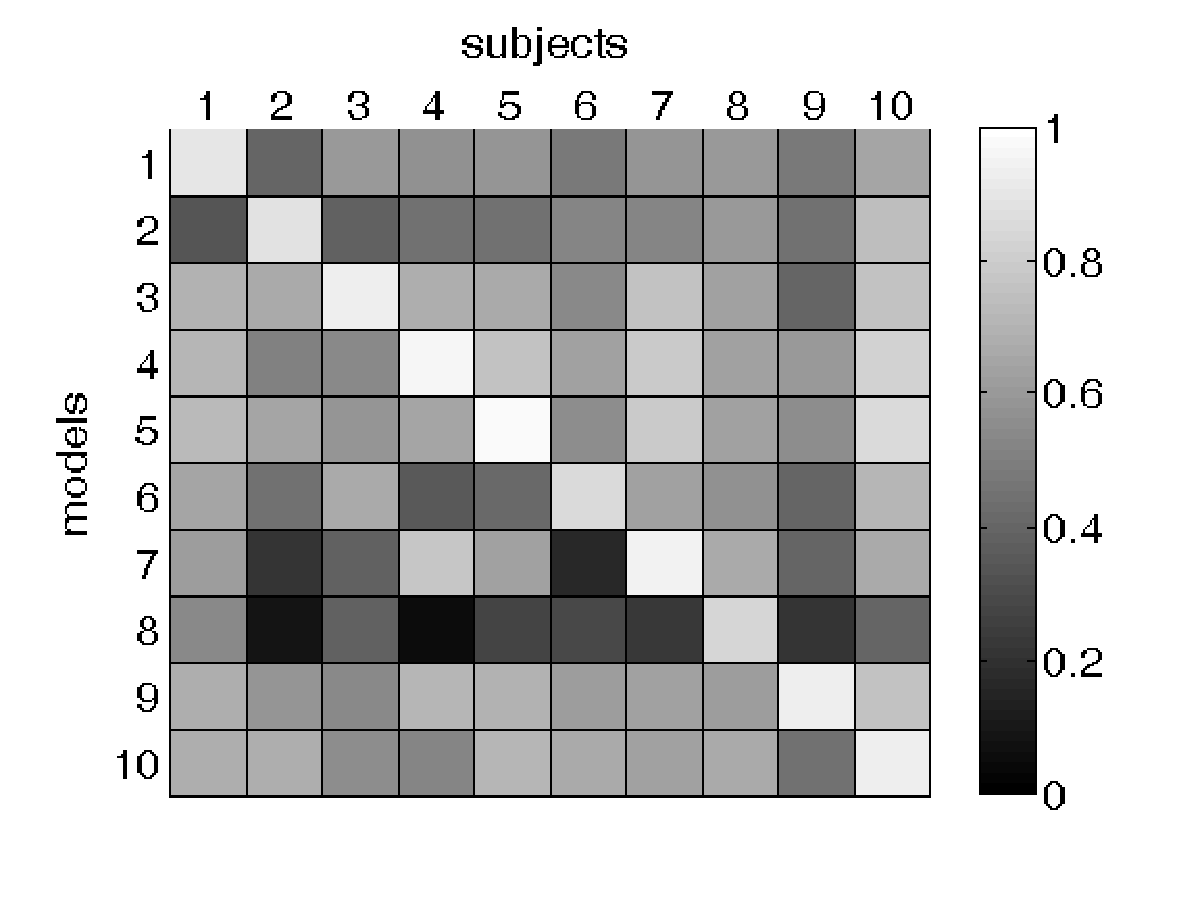
\includegraphics[width=0.45\textwidth]{crossRegr2.eps} \\
%    $0.60 \pm 0.18$ & $0.58 \pm 0.19$ \\
%  \end{tabular}
%  \caption{cross-subject performance matrices, for classification (top
%    row) and regression (bottom row), in the SA (left column)
%    and FA phase (right column); the numbers refer to all element of
%    the matrices, excluding the diagonals.}
%  \label{fig:cross}
%\end{figure*}

The overall results indicate that a large amount of the models
overlap, or at least that there is a certain cross-subject capacity of
prediction. Consider the numbers below the matrices in the Figure: in
classification, the performances are $51.69\%$ and $54.04\%$, with the
remarkable particular that the FA-models are slightly, but
consistently, \emph{better} in cross-subject analysis (higher mean
values and lower standard deviations) than the SA-models. This
indicates that, as already hinted at in the previous Subsection, the
FA-models have a wider knowledge of the respective input spaces and,
therefore, of the input space \emph{tout court}. This gives them a
little edge over the more limited SA-models.

As far as regression is concerned, things are even better, the average
cross-subject correlation being around $0.60$. To some extent, it is
likely that some of these models could actually be used as bootstrap
models for training online on new subjects. This corroborates the
hypothesis that, given a sufficiently large number of subjects, a
``common model'' could be potentially extracted, which would act as a
basis for online learning. How to build this common model is the
object of future research. Notice that, interestingly, models trained
on subjects $6$ (for the SA phase) and $8$ (FA phase) appear to be
particularly bad in predicting other subjects' data (the related rows
of the bottom left and right matrices, in turn, are rather darker than
the average).

Here the question naturally arises: what makes a model more or less
effective on ``new'' data? \footnote{this question is actually
connected to the general problem of generalisation in machine
learning; here we have no pretence of solving this problem in general,
but only to give a hint at the solution in this particular framework.}
In our previous work, we showed a significant (inverse) correlation
between the performance matrices and the \emph{cross-distance
matrices} $D$, obtained by evaluating a mean distance $D_{ij}$ between
two sample sets $S_i$ and $S_j$ like this:

$$ D_{ij} = \frac{1}{|S_j|} \sum_{s_j \in S_j}{\min_{s_i \in S_i}{ ||s_j-s_i||^2 } } $$

Here we repeat the analysis for each pair $(i,j)$ of subjects and for
the two phases and problems. The results show that inverse correlation
is absent in the case of the FA phase in classification; it is mild
($-0.32$) for SA in classification; and that it is strong in the case
of regression ($-0.63$ for the SA phase and $-0.65$ for the FA
phase). It is likely that the correlation in regression is connected
to the actual smoothness of the function the system is trying to
approximate --- a consideration which we already put forward in the
previous work. It is unclear why the classification problems show a
weak correlation or none at all.

\section*{Conclusions}
\label{sec:discussion}
  
Our results clearly indicate that the problem, at least from a
theoretical point of view, is solved for healthy subjects. The
indicated approach, that is, Support Vector Machines, obtains
excellent results in all variants hereby presented. This does not
mean, of course, that SVMs are the one and only good method; actually,
Neural Networks are LWPR (see \cite{lwpr}) have already been employed
with only slightly worse results, and probably even simpler approaches
would get an acceptable level of performance.

This paper, as already said, is a companion to, and the natural
extension of, \cite{2008.ICRA,2008.BioCyb}. Here we show that the
approach described therein can be applied with sucess to any healthy
subject, and in a non-controlled, DLA-like framework. We also show
that the uniformisation procedure produces remarkably small training
sets, which nevertheless attain an excellent accuracy, and we confirm
the phenomenon therein described, consisting in a linear degradation
of the performance, as the minimum distance $d$ is linearly changed,
whereas the training set size changes polynomially.

We are now ready to claim that machine learning can be used in a
practical application of this framework, at least on healthy subjects,
to realise an adaptive approach to EMG-based control of mechanical
hands. As far as ``real'' prosthetics is concerned, we have already
carried on experiments on amputees, revealing that a surprisingly fine
residual muscular activity can be found in stumps, even several
\emph{decades} after the operation (see our poster
\cite{2008.Neurorob}; a full report is in preparation). Muscular
plasticity means highly discernible signals, and a system such as the
one described here is then able to solve the problem in that case,
too.

The possibility of building a common model to aid reciprocal learning
is fascinating. In this paper we have shown that it should be possible
to build one without much effort; a combination of data taken from
other patients, together with the uniformisation strategy, could
actually give a head-start to the prosthesis, therefore shortening the
patient's training time.

All in all, we believe that the new, exciting scenario of
\emph{adaptive prosthetics} is ready to appear. In such a scenario,
the patient and the prosthesis are involved in a loop of
\emph{reciprocal learning} and the training time is dramatically
shorter than it is now. At the same time, the amputee can control the
prosthesis in a much finer way, allowing for a better restoration of
pre-operation DLA capacity. This will change in a better way the
amputees' life. The method can be, in principle, extended to other
kinds of amputation and disability.

\section*{Competing interests}

No competing interests at all.

\section*{Authors contributions}

CC has collected some data, performed the data analysis and written most of the paper. AEF has taken care of the setup, collected most of the data and written some of the paper. GS has helped design the experiment, proof-read the paper and given useful advice throughout the realisation of the work. All authors have read and approved the manuscript.

\section*{Acknowledgements}

This work has been partially supported by the EU project NEURObotics, FP6-IST-001917.

{\ifthenelse{\boolean{publ}}{\footnotesize}{\small}
 \bibliographystyle{bmc_article}  % Style BST file
  \bibliography{paper,claudio} }     % Bibliography file (usually '*.bib' ) 

\ifthenelse{\boolean{publ}}{\end{multicols}}{}

\section*{Tables}

\begin{table}[!ht] \centering
  \caption{Mean values and standard deviations of the hyperparameters $\gamma$ and $C$.}
  \begin{tabular}{|c|r|r|}
    \hline
    Phase, problem & $log_{10}(\gamma)$ & $log_{10}(C)$ \\
    \hline
    SA, class.     & $-0.35 \pm 0.58$   & $1.6  \pm 0.84$ \\
    FA, class.     & $-0.65 \pm 0.54$   & $1.55 \pm 0.83$ \\
    SA, regr.      & $-0.50 \pm 0.24$   & $1.45 \pm 0.44$ \\
    FA, regr.      & $-0.60 \pm 0.26$   & $1.45 \pm 0.37$ \\
    \hline
  \end{tabular}
  \label{tab:hyp}
\end{table}

\section*{Figure legends}

\begin{figure}[!ht] \centering
%  \begin{center}
%  \begin{tabular}{ccc}
%    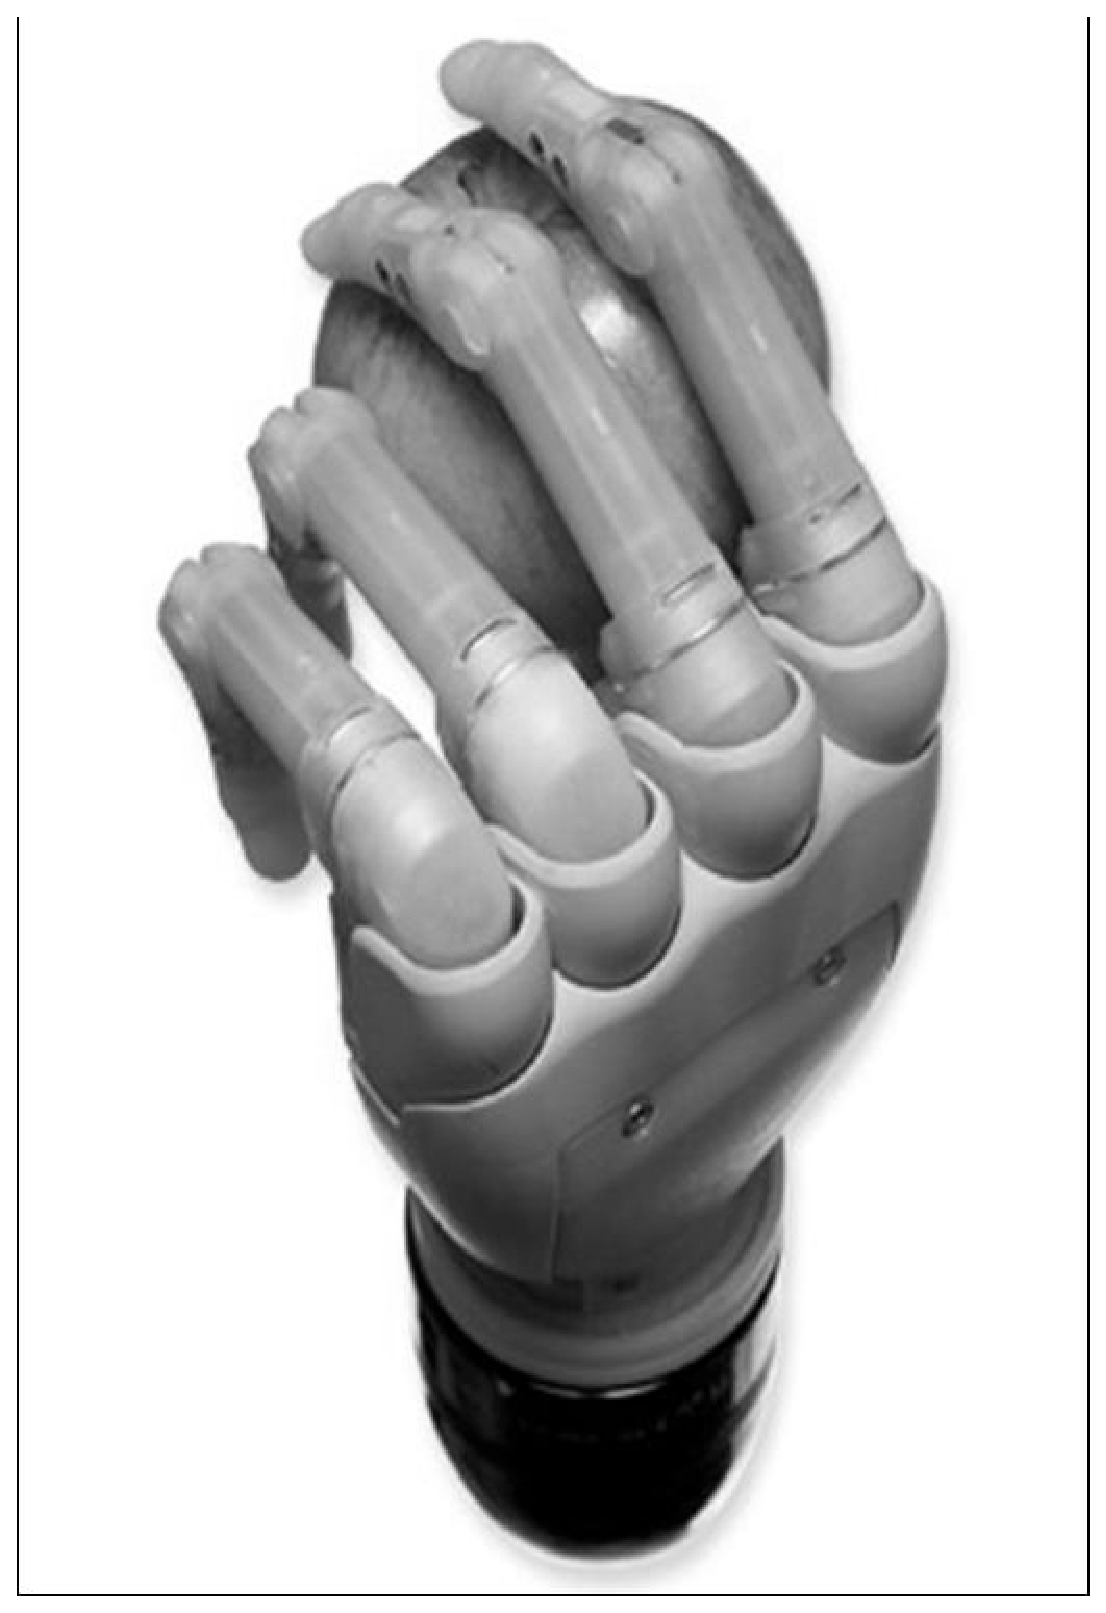
\includegraphics[width=0.25\textwidth]{hands_TB.eps} &
%    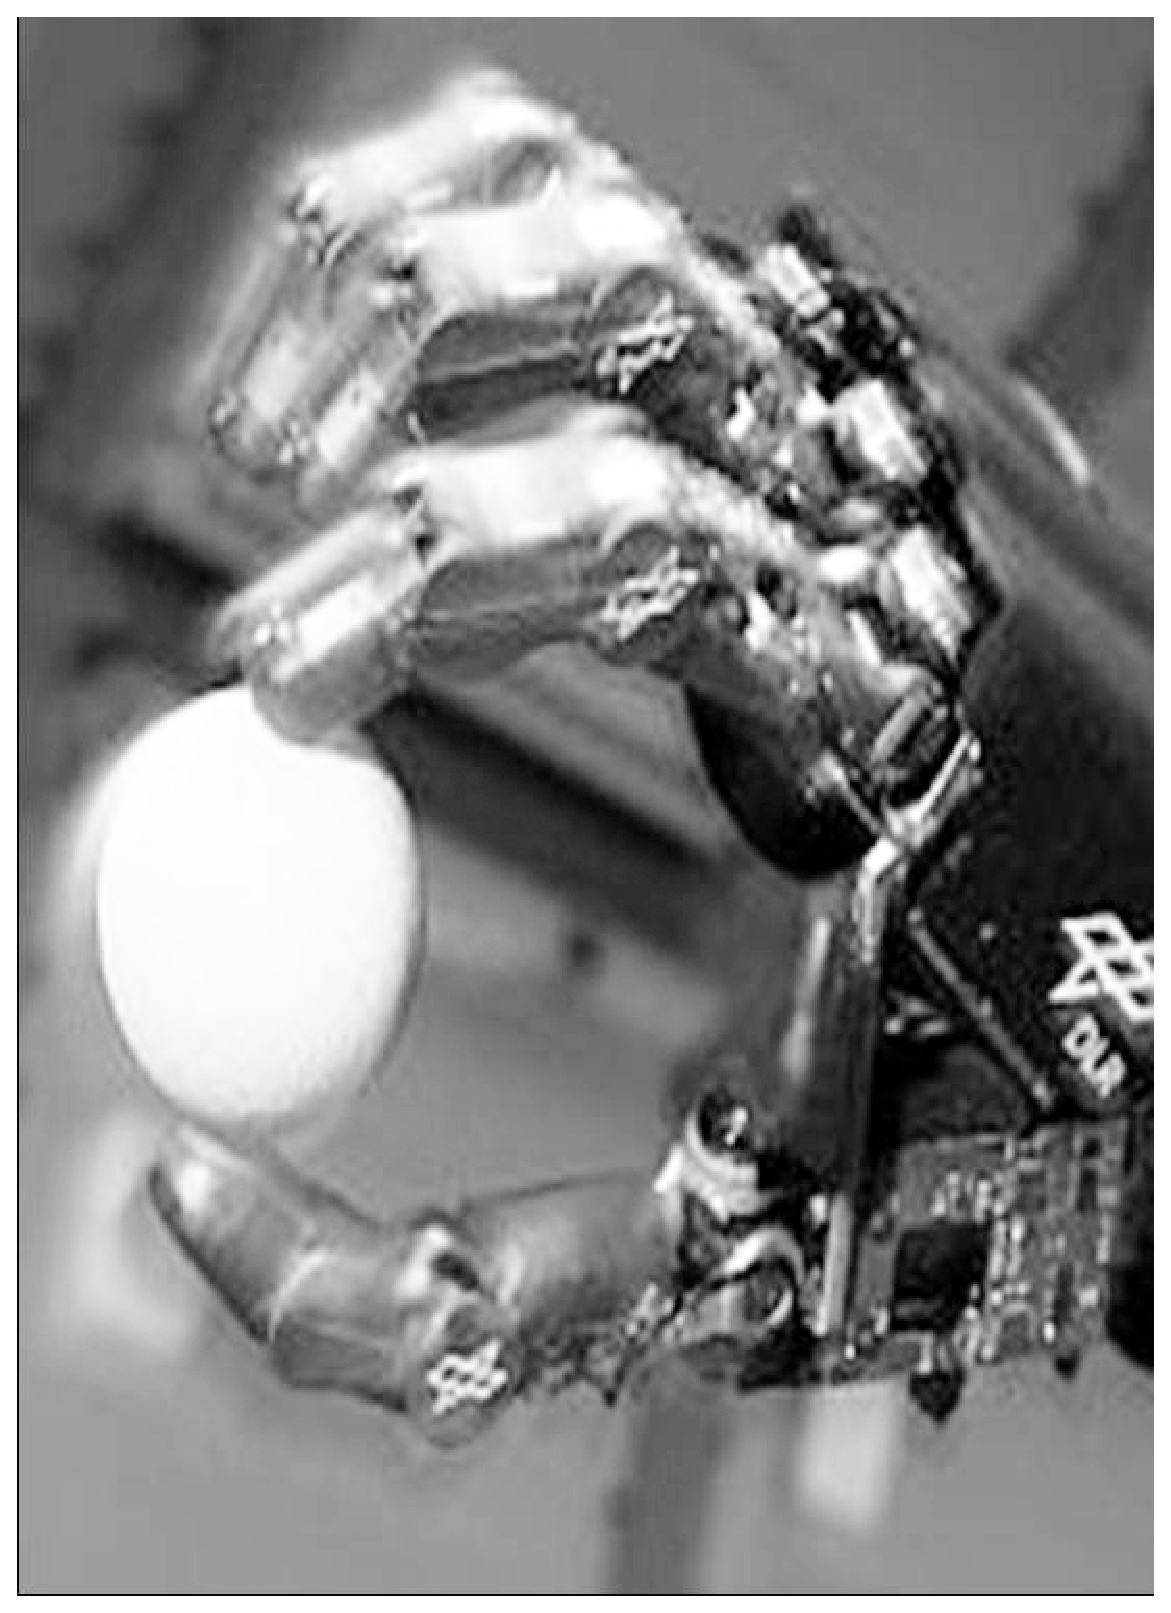
\includegraphics[width=0.25\textwidth]{hands_DLRII.eps} &
%    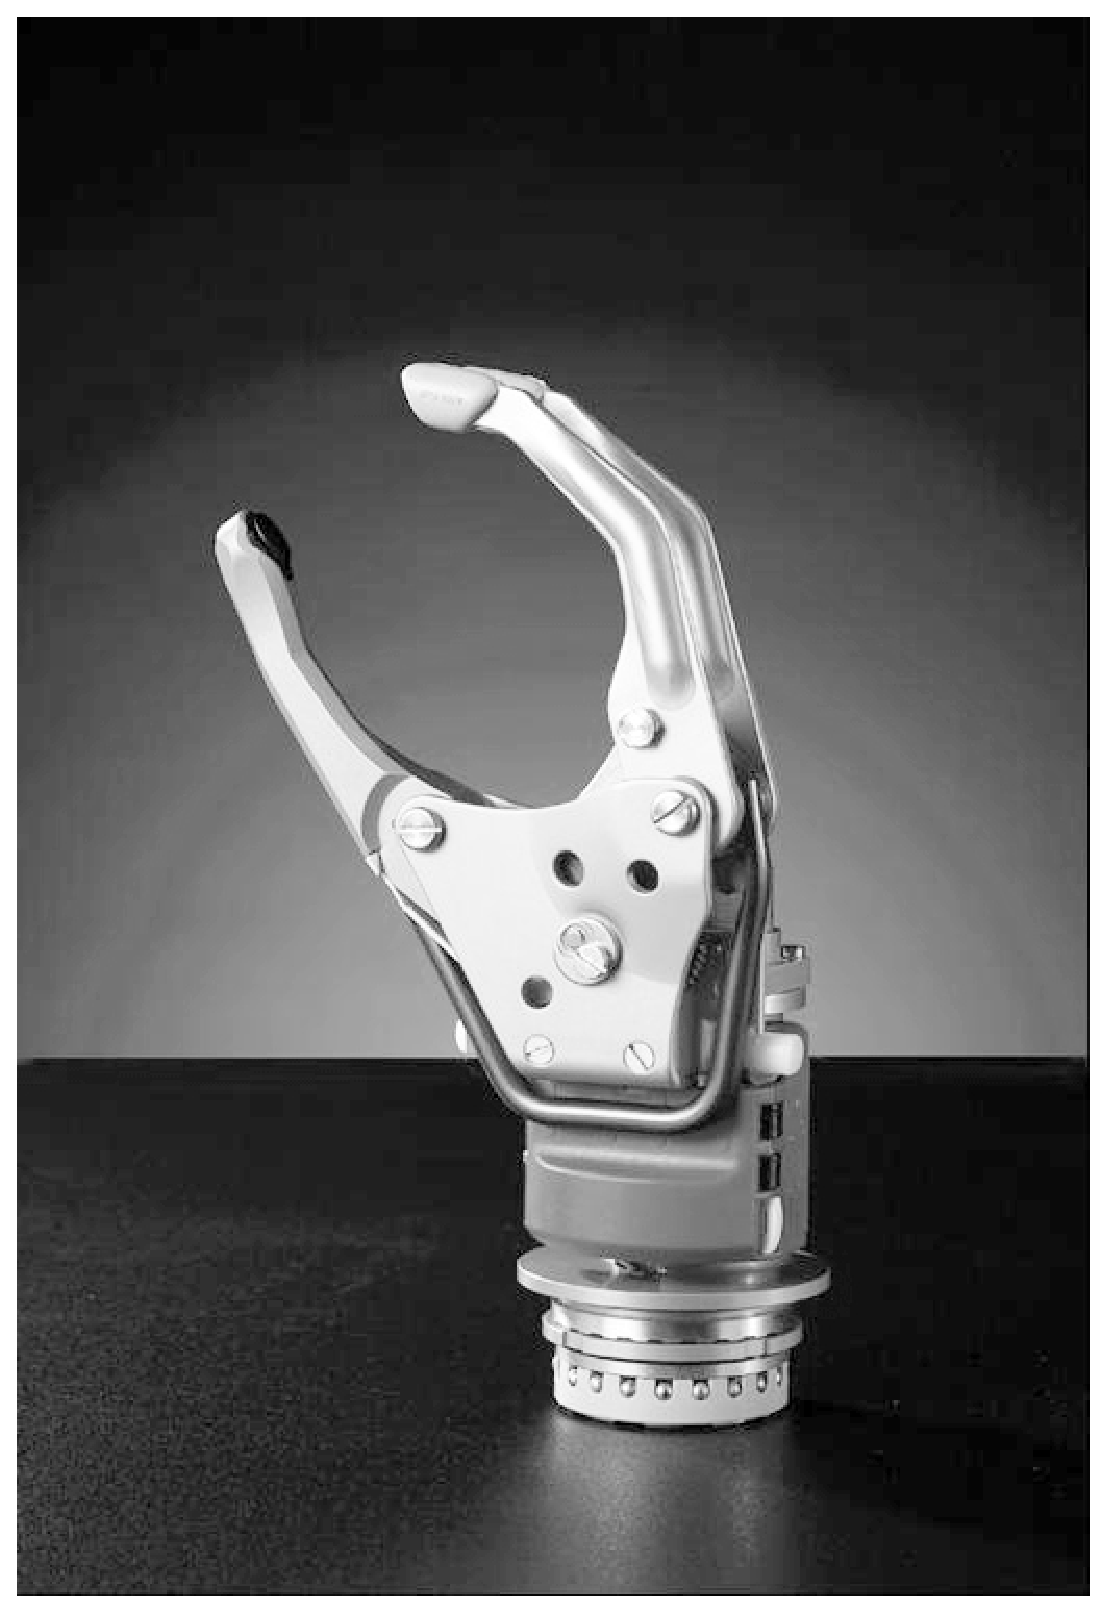
\includegraphics[width=0.25\textwidth]{hands_OB.eps} \\
%    $(a)$ & $(b)$ & $(c)$
%  \end{tabular}
%  \end{center}
  \caption{$(a)$ Touch Bionics's i-LIMB prosthetic hand (reproduced
    from \cite{ilimb}); $(b)$ the DLR-II mechanical hand; $(c)$ Otto
    Bock's SensorHand Speed (reproduced from \cite{sensorhand}).}
  \label{fig:hands}
\end{figure}

\begin{figure}[!ht] \centering
%  \begin{tabular}{ccc}
%    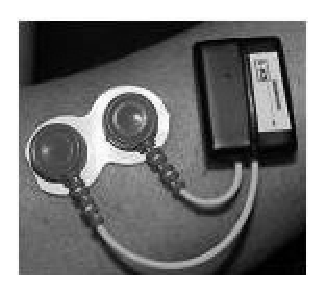
\includegraphics[height=0.16\textheight]{Electrode.eps} &
%    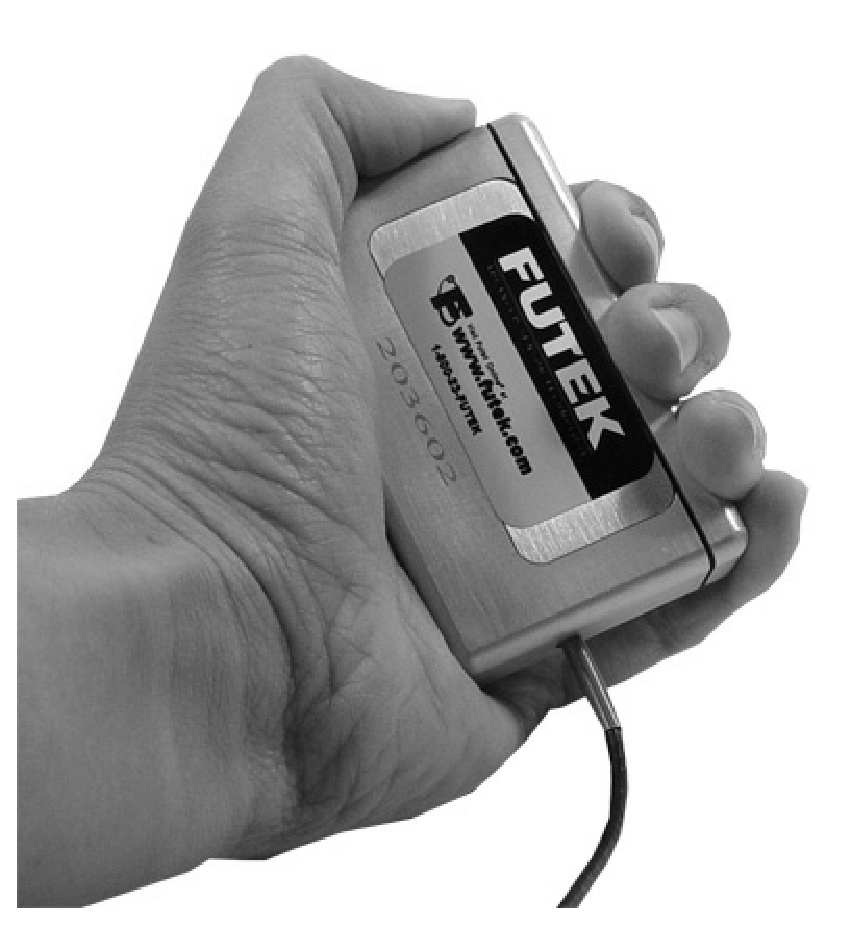
\includegraphics[height=0.16\textheight]{Hand_Gripper.eps} &
%    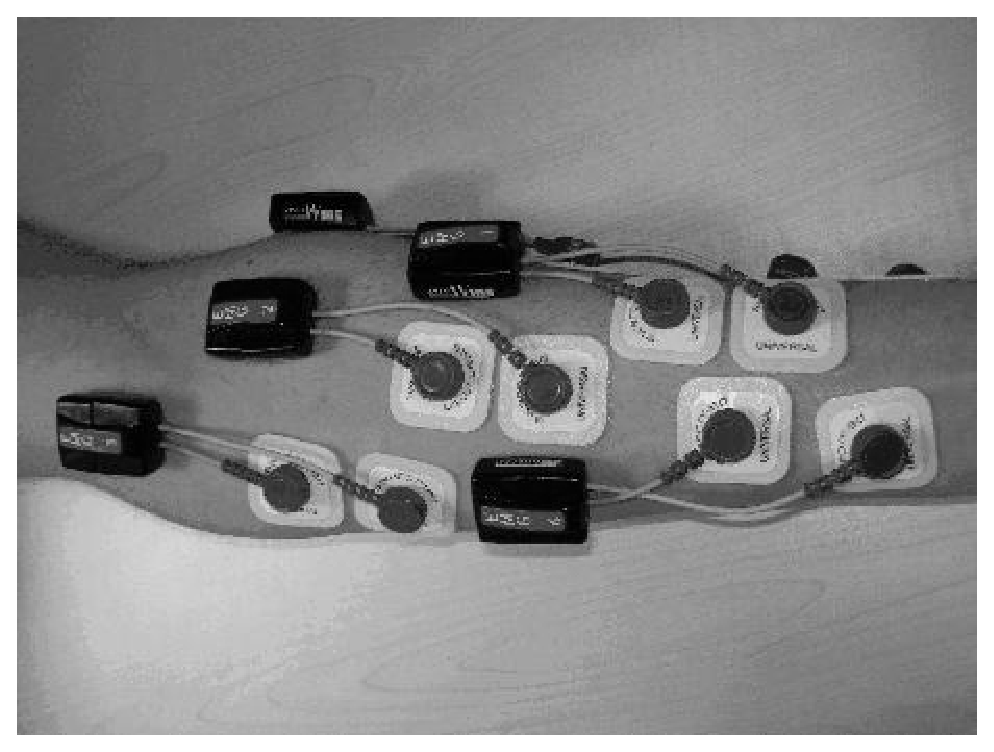
\includegraphics[height=0.16\textheight]{El_Arrangement.eps} \\
%    $(a)$ & $(b)$ & $(c)$ \\
%  \end{tabular}
  \caption{The experimental setup (\textit{subject side}): $(a)$ an EMG
    wireless electrode; $(b)$ the FUTEK force sensor; $(c)$ the typical
    placement of the EMG electrodes on a subject's forearm (ventral side).}
  \label{fig:SubjSetup}
\end{figure}

\begin{figure}[!ht] \centering
%  \begin{tabular}{cc}
%    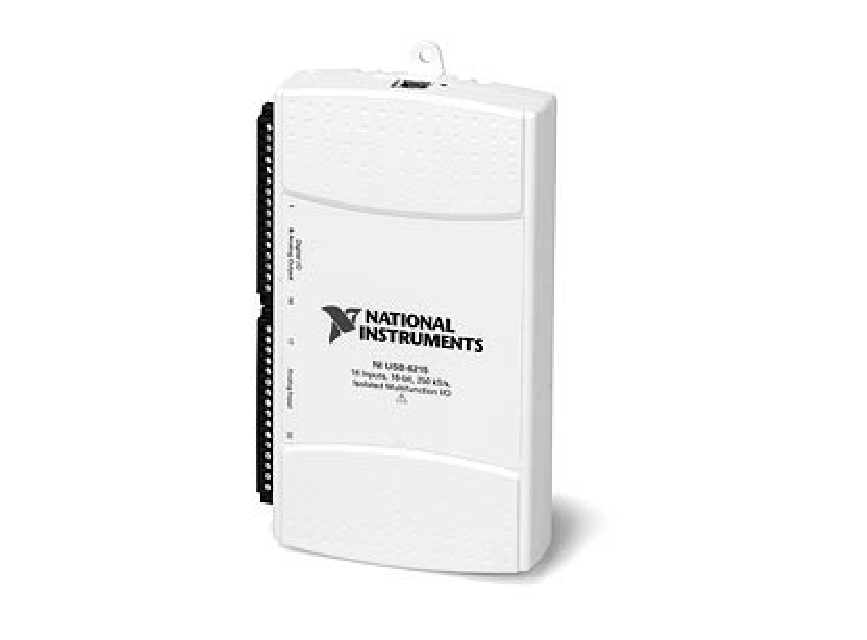
\includegraphics[height=0.16\textheight]{NI-6211.eps} &
%    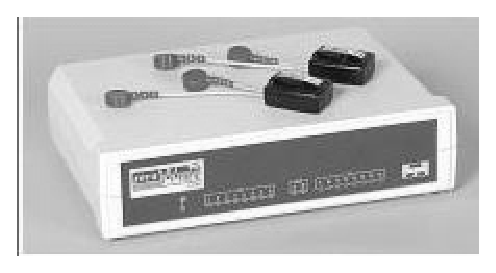
\includegraphics[height=0.16\textheight]{Zero_Base.eps} \\
%  $(a)$ & $(b)$\\
%  \end{tabular}
  \caption{The experimental setup (\textit{experimenter side}): $(a)$
   the USB data acquisition card (NI-USB6211); $(b)$ the EMG device
   receiver.}
  \label{fig:ExpSetup}
\end{figure}

\begin{figure}[!t] \centering
%  \begin{tabular}{ccc}
%    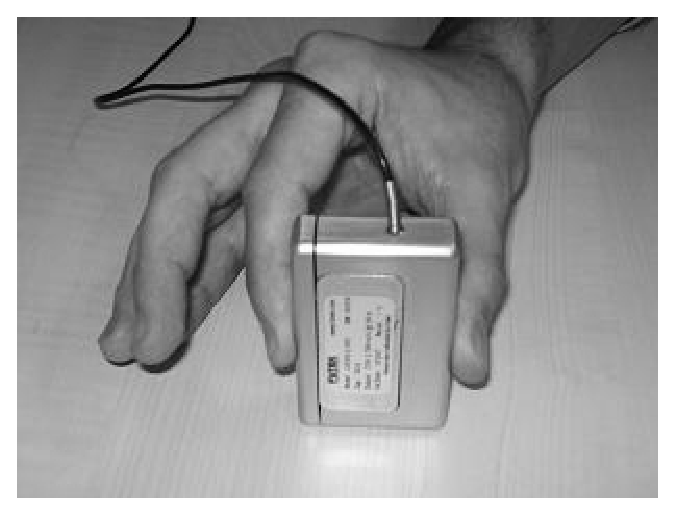
\includegraphics[height=0.16\textheight]{grip1.eps} &
%    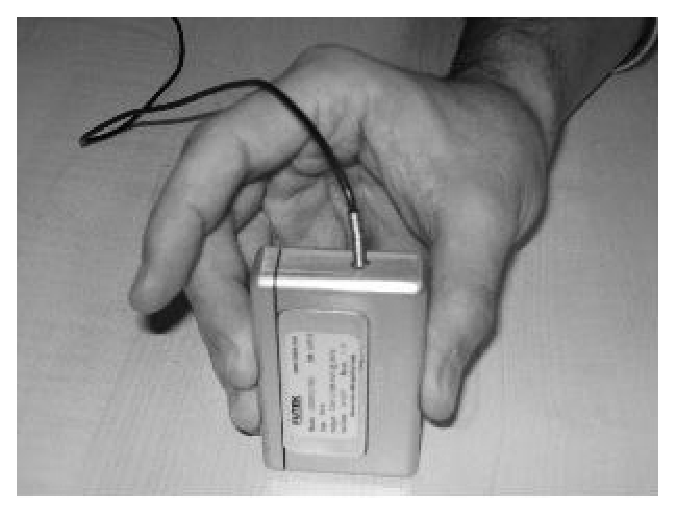
\includegraphics[height=0.16\textheight]{grip2.eps} &
%    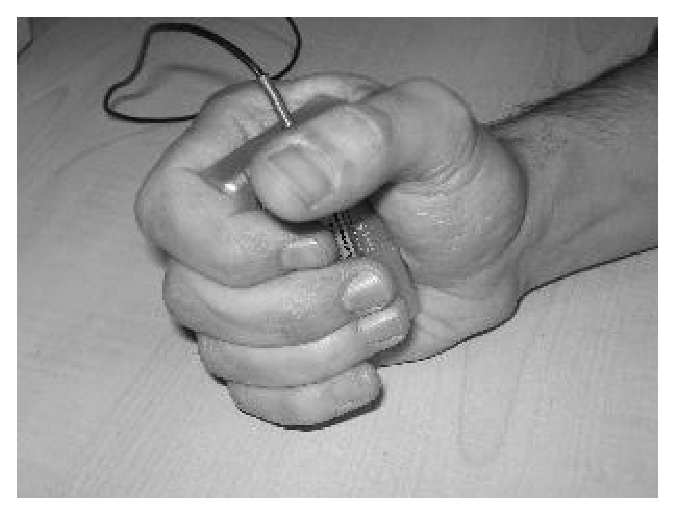
\includegraphics[height=0.16\textheight]{grip3.eps} \\
%    $(a)$ & $(b)$ & $(c)$ \\
%  \end{tabular}
  \caption{The three different grips employed in the experiment: $(a)$
   index precision grip; $(b)$ other fingers precision grip; $(c)$
   power grasp.}
  \label{fig:Grasps}
\end{figure}

\begin{figure}[!ht] \centering
%  \begin{tabular}{cc}
%    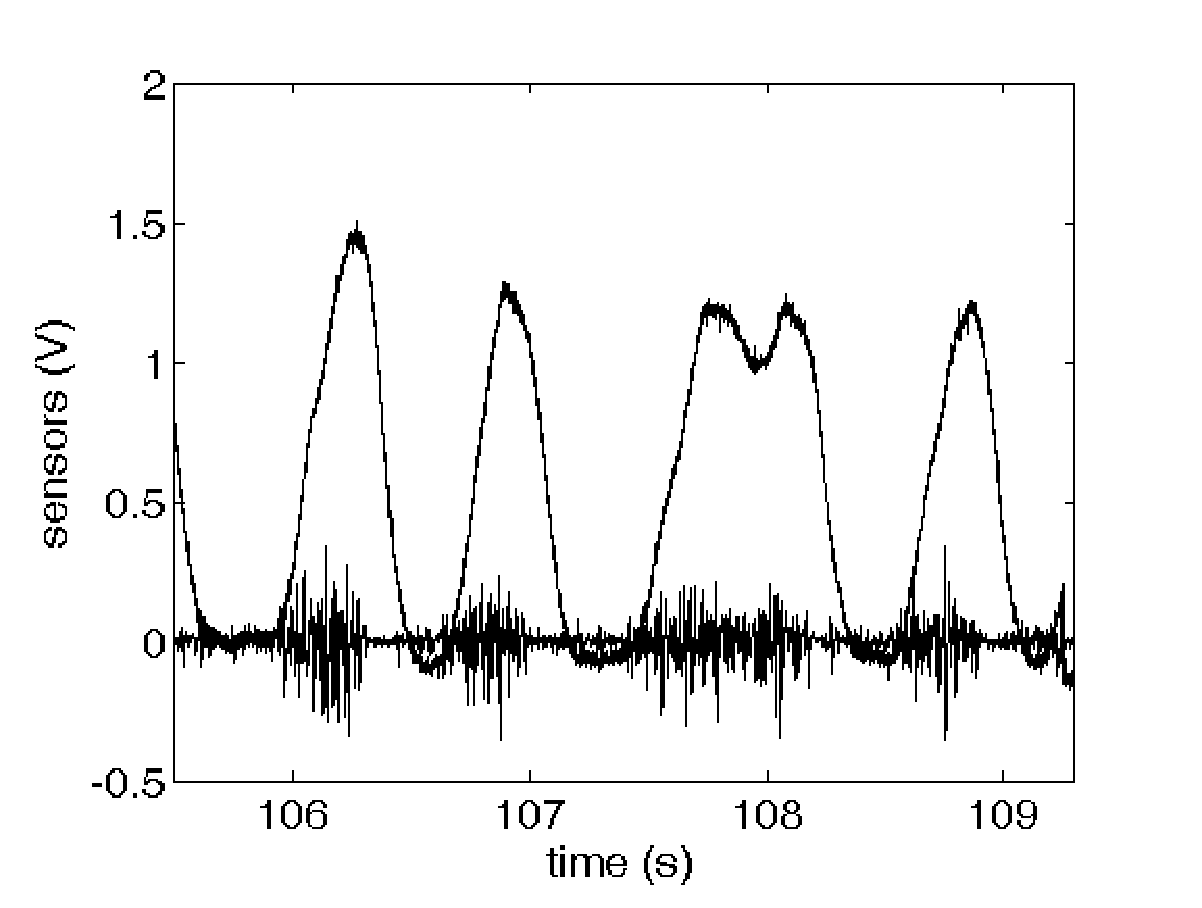
\includegraphics[width=0.45\textwidth]{force_raw.eps} &
%    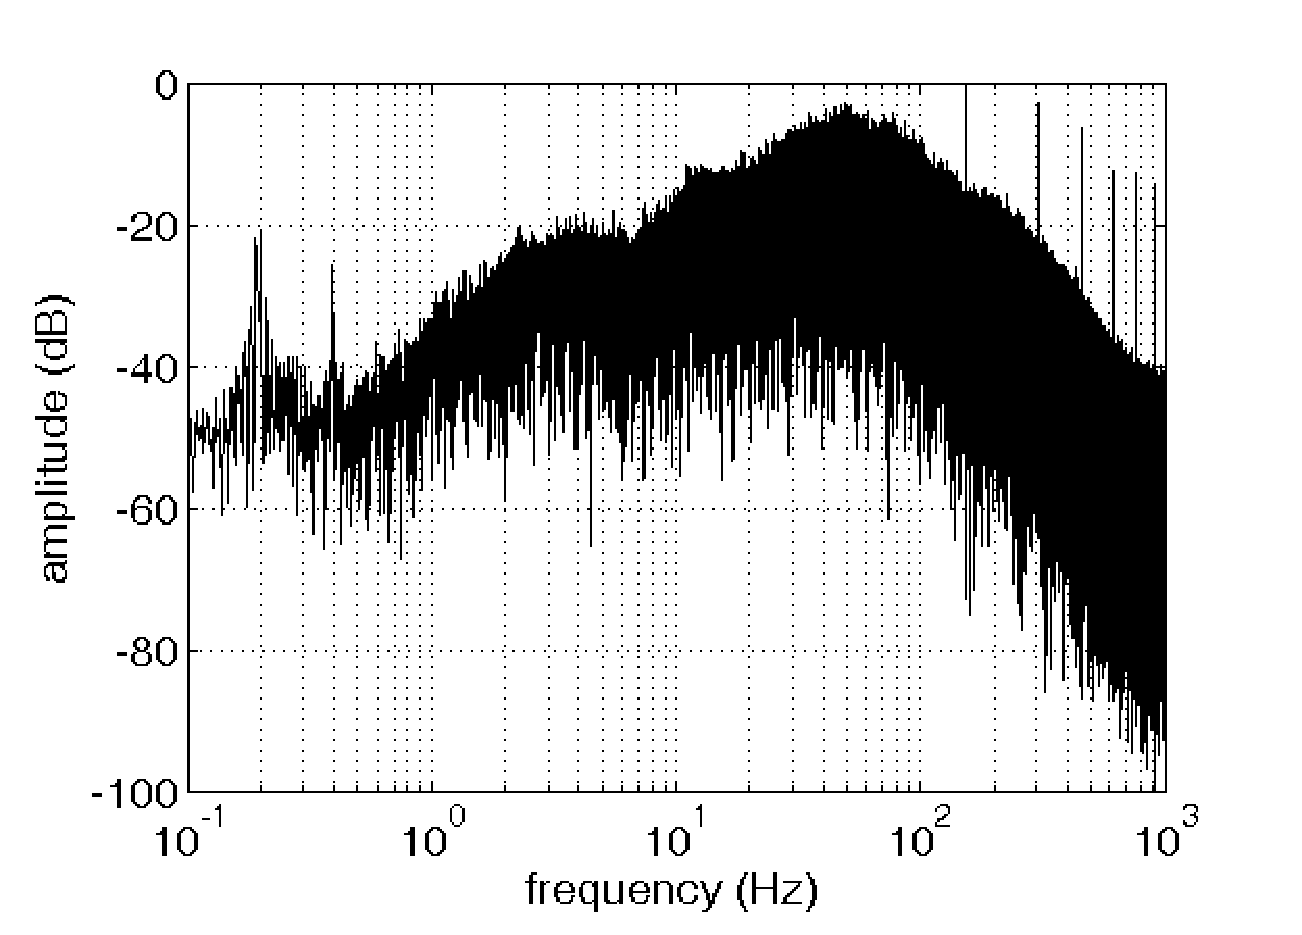
\includegraphics[width=0.45\textwidth]{spectrum_raw.eps} \\
%    $(a)$ & $(b)$ \\
%  \end{tabular}
  \caption{$(a)$ typical raw EMG and force signals (the EMG signal
    being the bottom, high-frequency one); $(b)$ frequency diagram of
    the EMG signal.}
  \label{fig:spectra}
\end{figure}

\begin{figure}[!ht] \centering
%  \begin{tabular}{ccc}
%    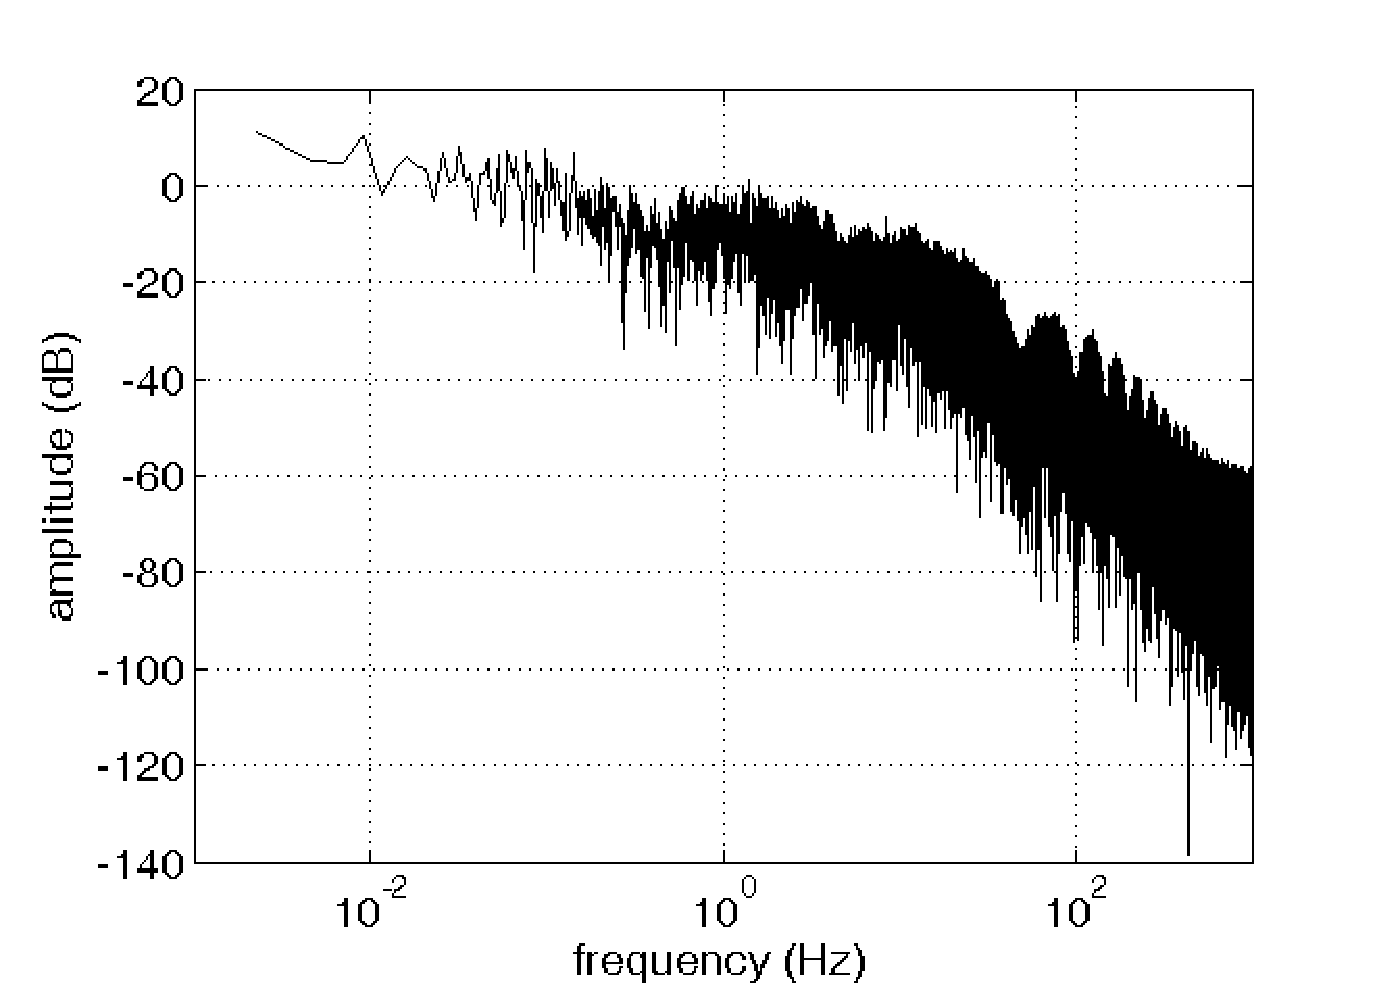
\includegraphics[width=0.3\textwidth]{spectrum_RMS0040.eps} &
%    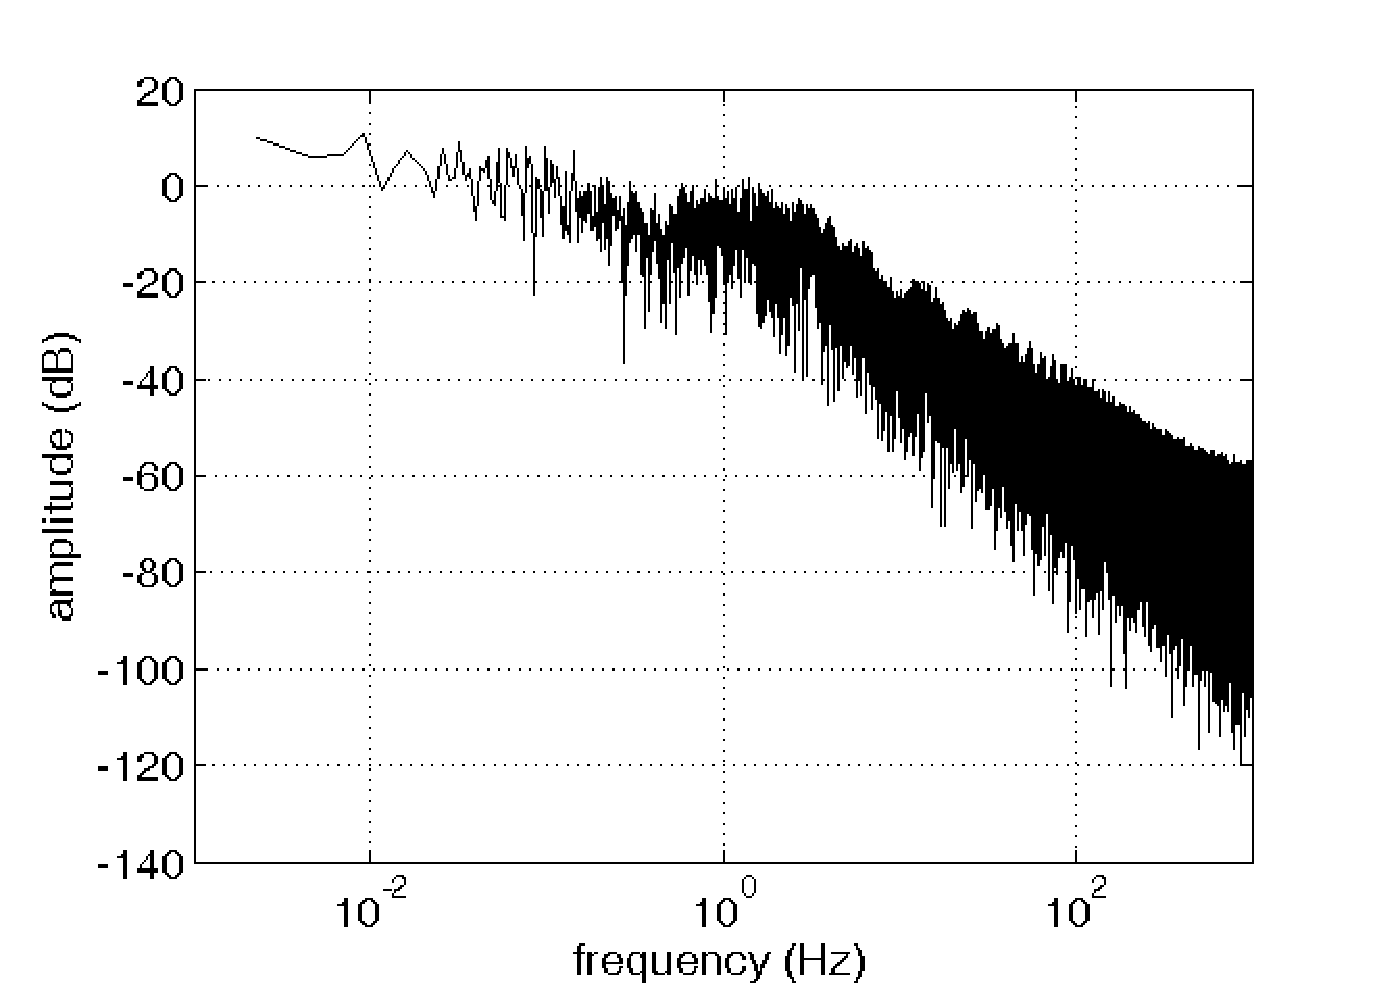
\includegraphics[width=0.3\textwidth]{spectrum_RMS0200.eps} &
%    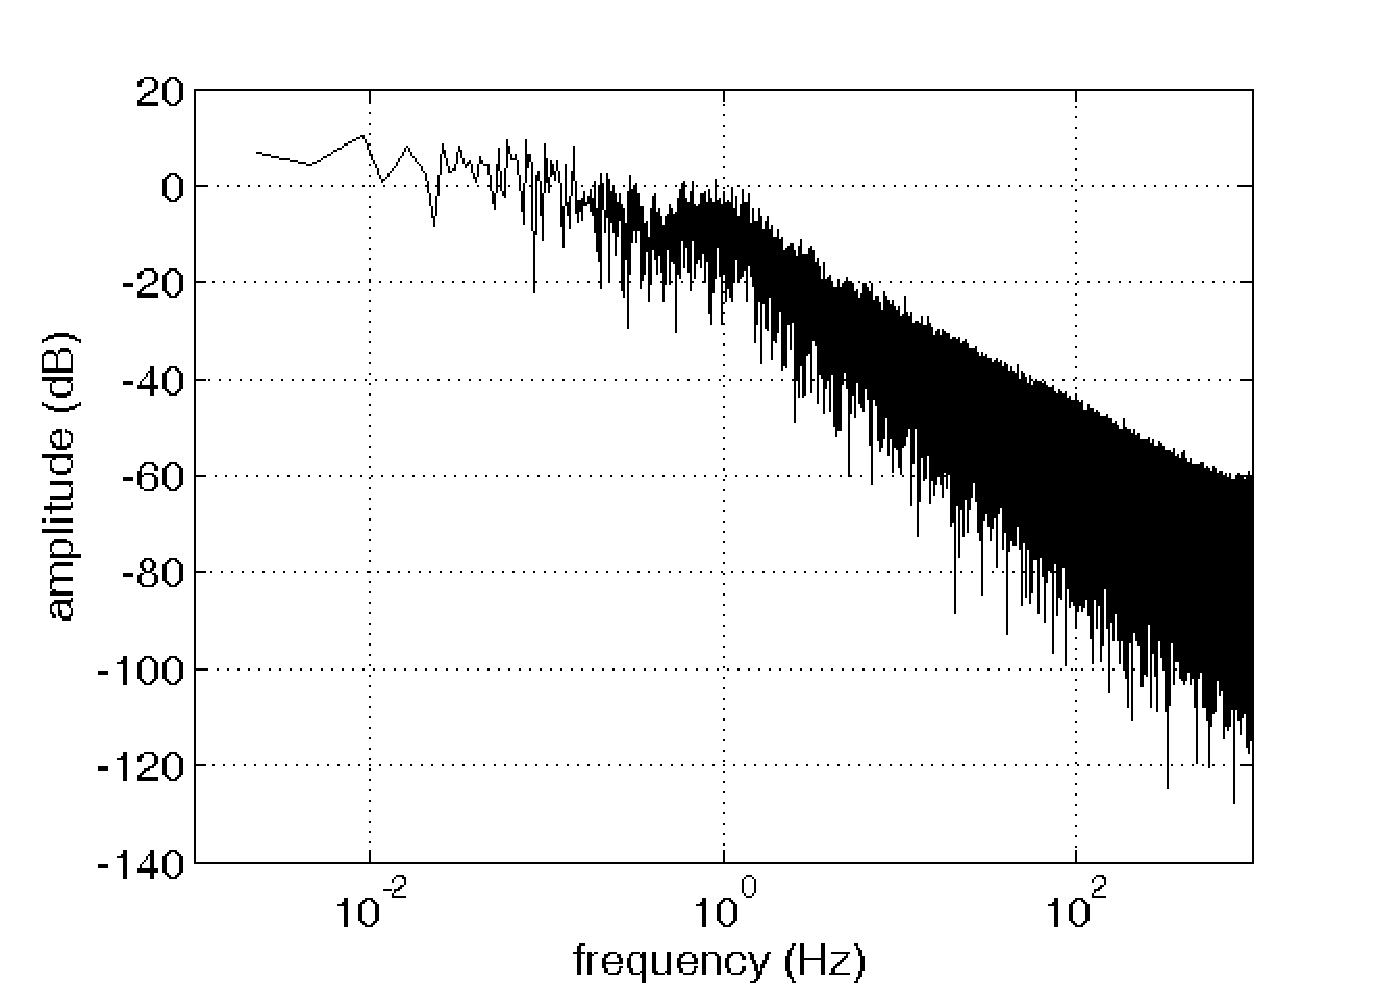
\includegraphics[width=0.3\textwidth]{spectrum_RMS1000.eps} \\
%    $(a)$ & $(b)$ & $(c)$ \\
%  \end{tabular}
  \caption{(left to right) effects of the RMS on the bandwidth of the EMG
    signals, for $T_{RMS} = 20, 100, 500ms$.}
  \label{fig:RMSs}
\end{figure}

\begin{figure}[!ht] \centering
%  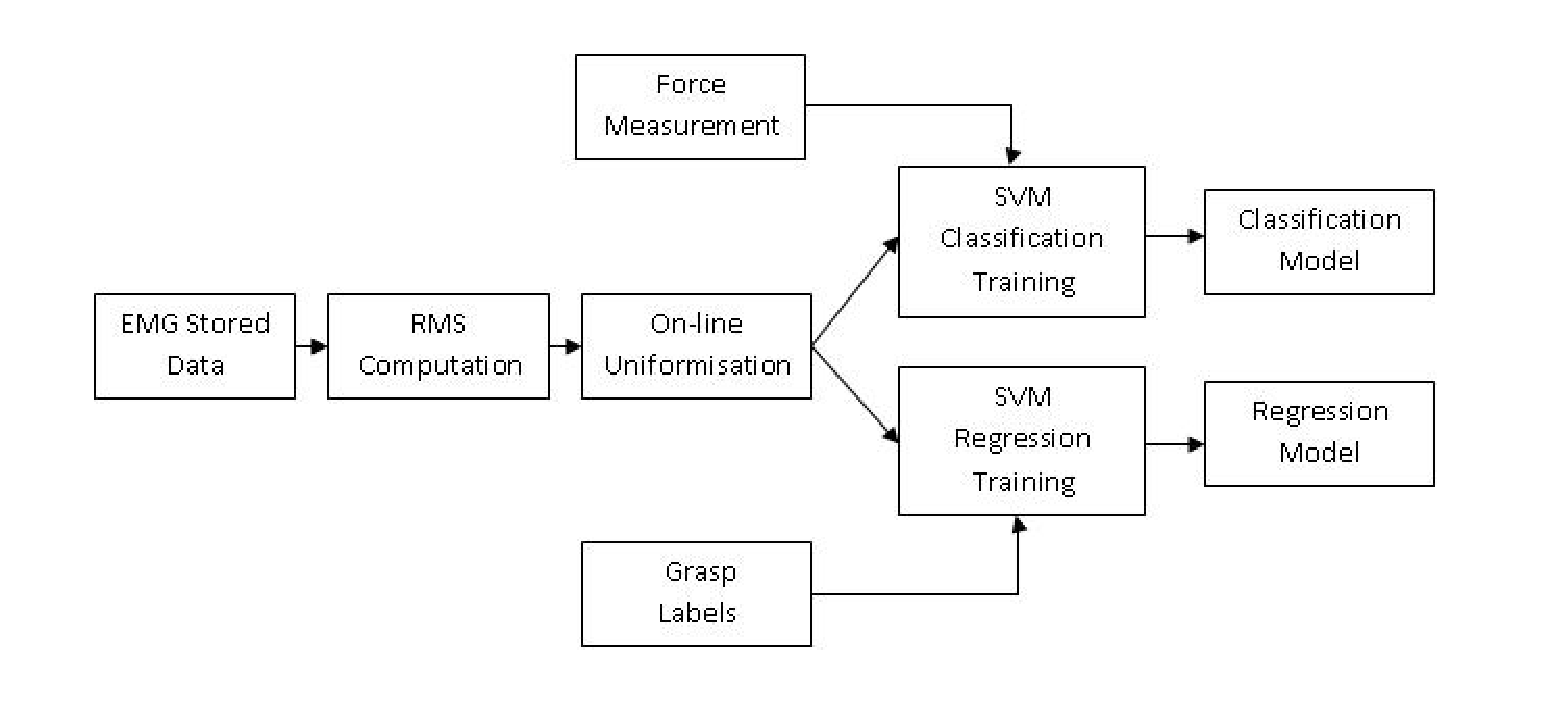
\includegraphics[width=0.75\textwidth]{Schema.eps} \\
  \caption{Graphical representation of the system employed to solve our problem.}
  \label{fig:Algorithm}
\end{figure}

\begin{figure}[!ht] \centering
%  \begin{tabular}{cc}
%    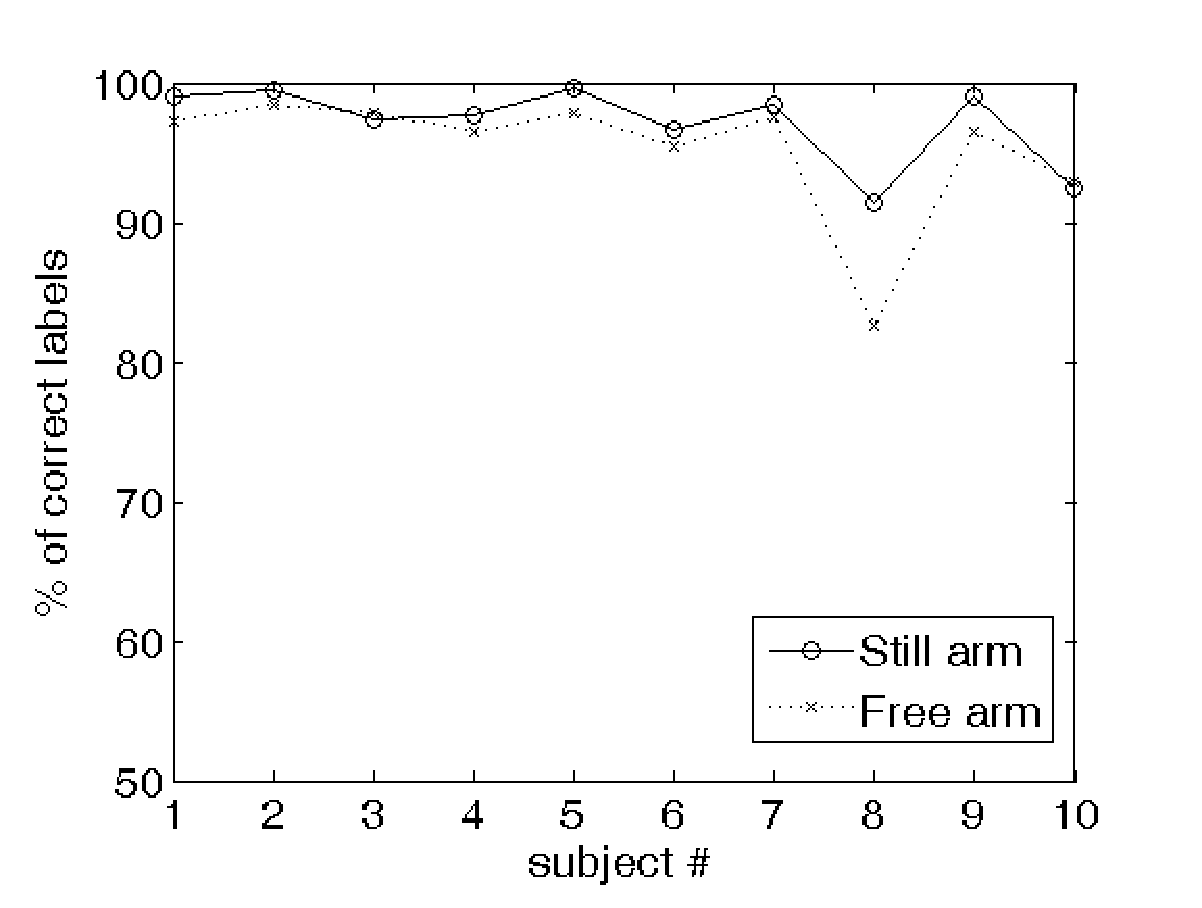
\includegraphics[width=0.45\textwidth]{perfClass.eps} &
%    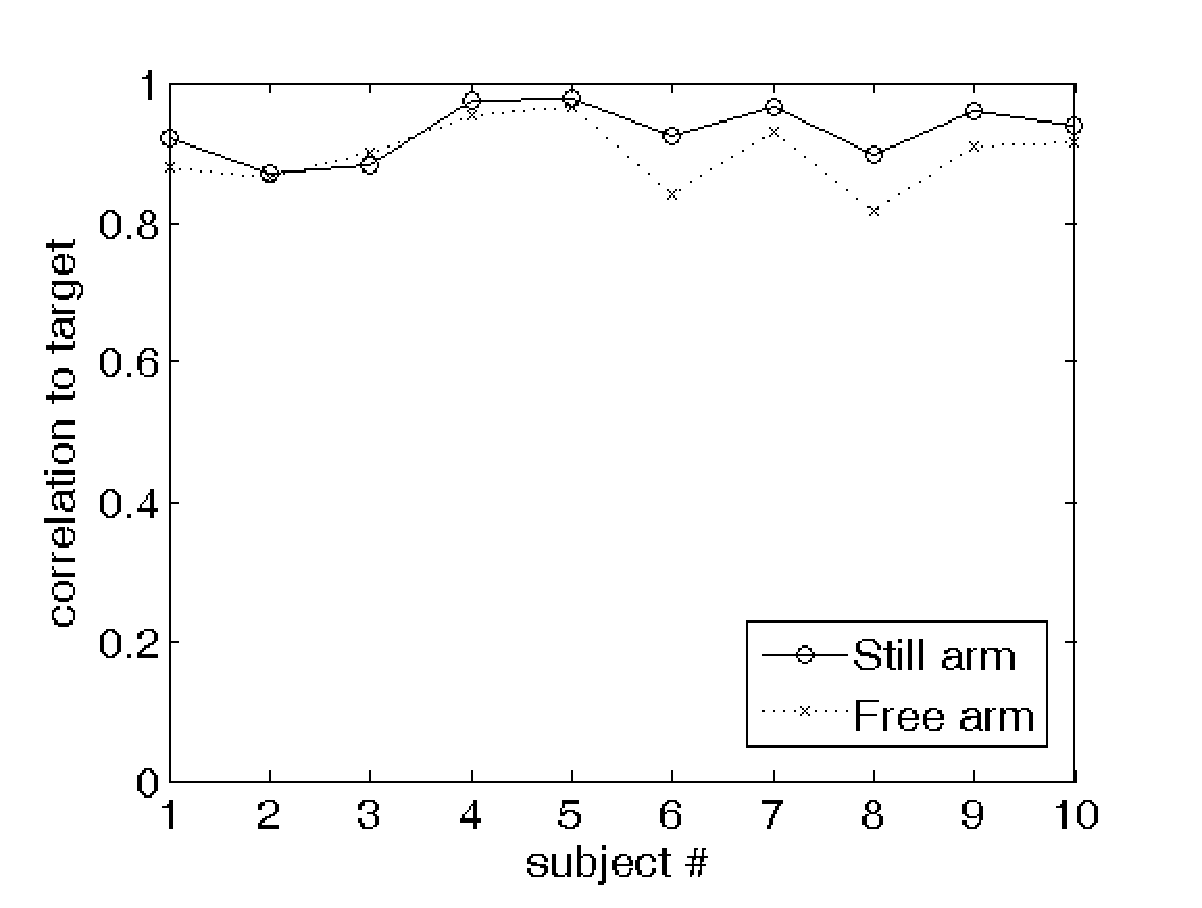
\includegraphics[width=0.45\textwidth]{perfRegr.eps} \\
%    $(a)$ & $(b)$ \\
%  \end{tabular}
  \caption{classification $(a)$ and regression $(b)$ results obtained
    by the system, on both phases of the experiment (FA and SA) and
    for each subject.}
  \label{fig:results}
\end{figure}

\begin{figure}[!ht] \centering
%  \begin{tabular}{cc}
%    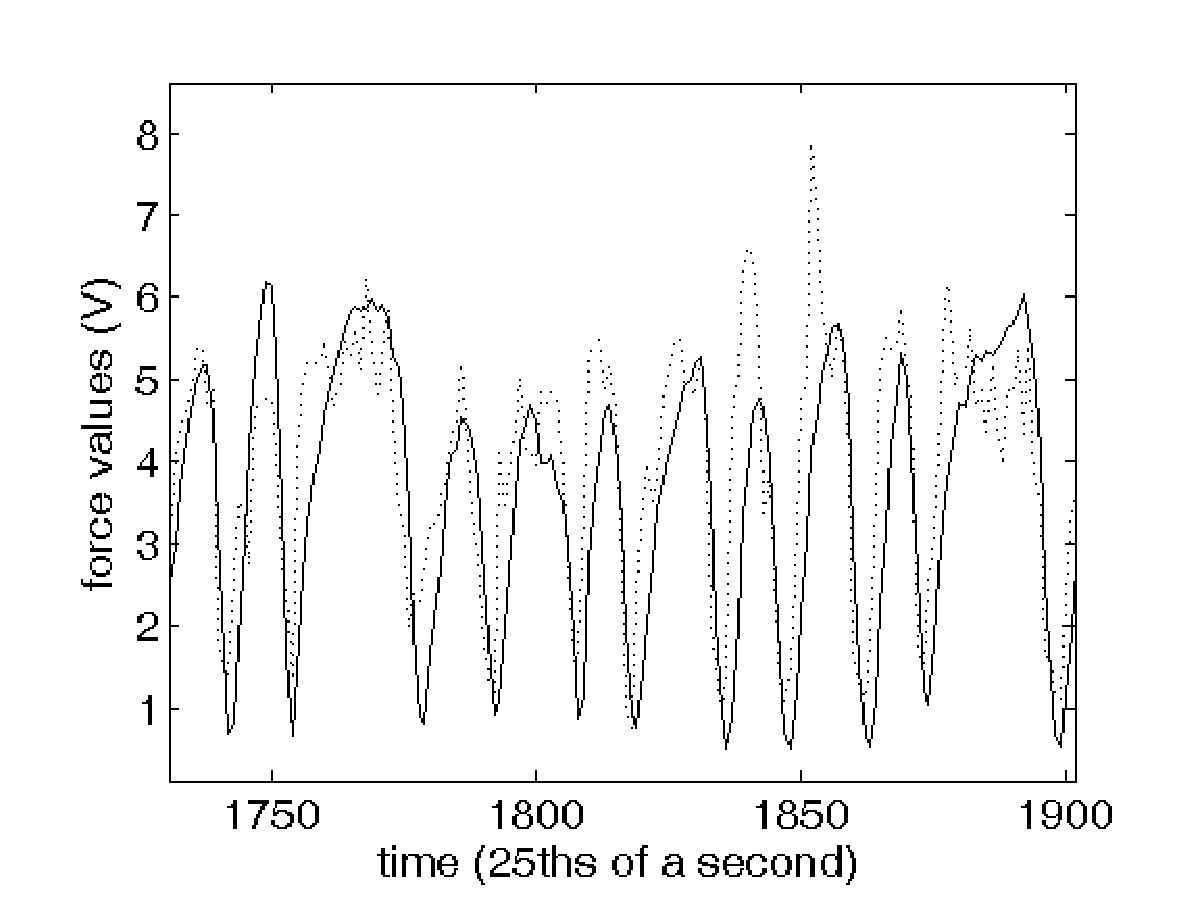
\includegraphics[width=0.45\textwidth]{example_6_one.eps} &
%    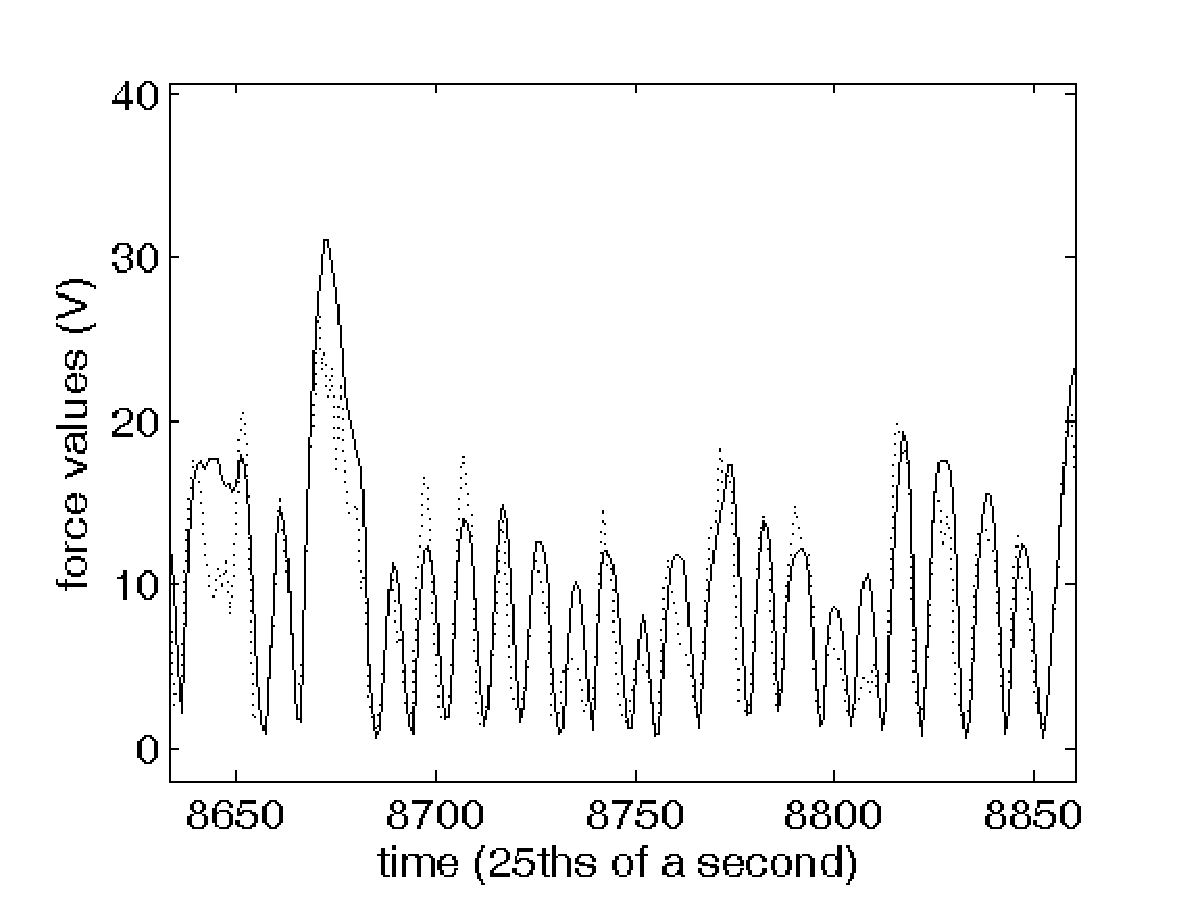
\includegraphics[width=0.45\textwidth]{example_6_two.eps} \\
%    $(a)$ & $(b)$ \\
%  \end{tabular}
  \caption{comparing true (continuous line) and guessed (dotted line) force values for regression of a
    typical subject (number $6$, FA phase).}
  \label{fig:examples}
\end{figure}

\begin{figure}[!ht] \centering
%  \begin{tabular}{cc}
%    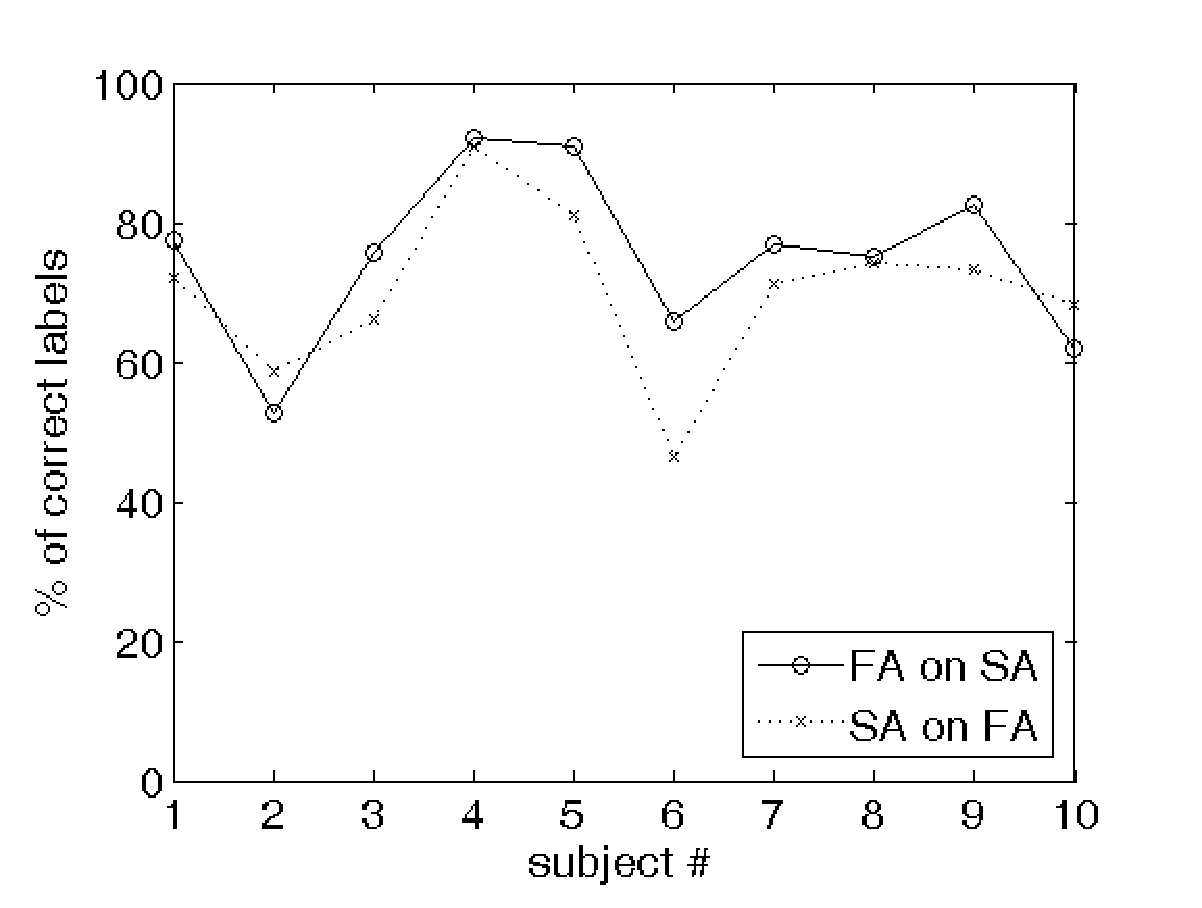
\includegraphics[width=0.45\textwidth]{2on1_class.eps} &
%    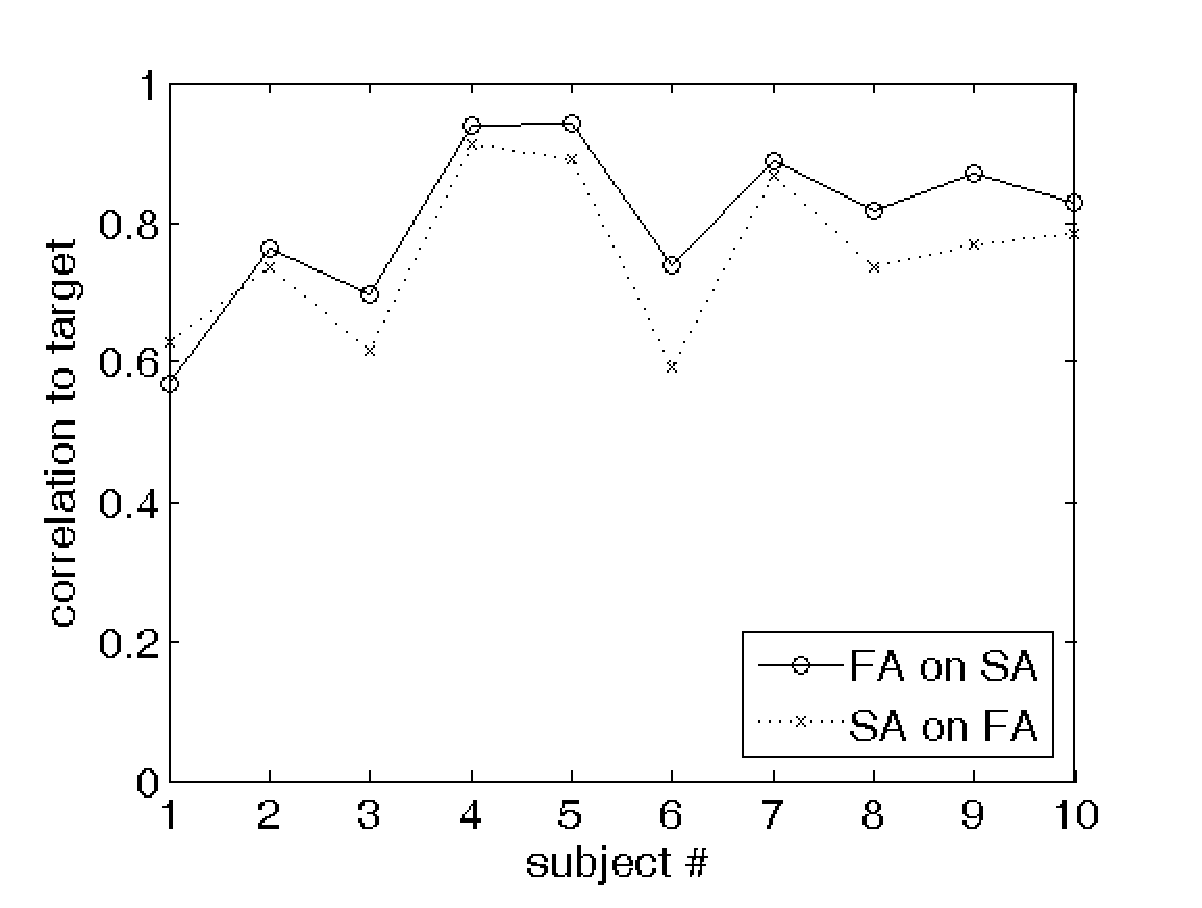
\includegraphics[width=0.45\textwidth]{2on1_regr.eps} \\
%    $(a)$ & $(b)$ \\
%  \end{tabular}
  \caption{classification $(a)$ and regression $(b)$ results obtained
    testing on SA-data models trained on FA, and vice-versa.}
  \label{fig:2on1}
\end{figure}

\begin{figure}[!ht] \centering
%  \begin{tabular}{c}
%    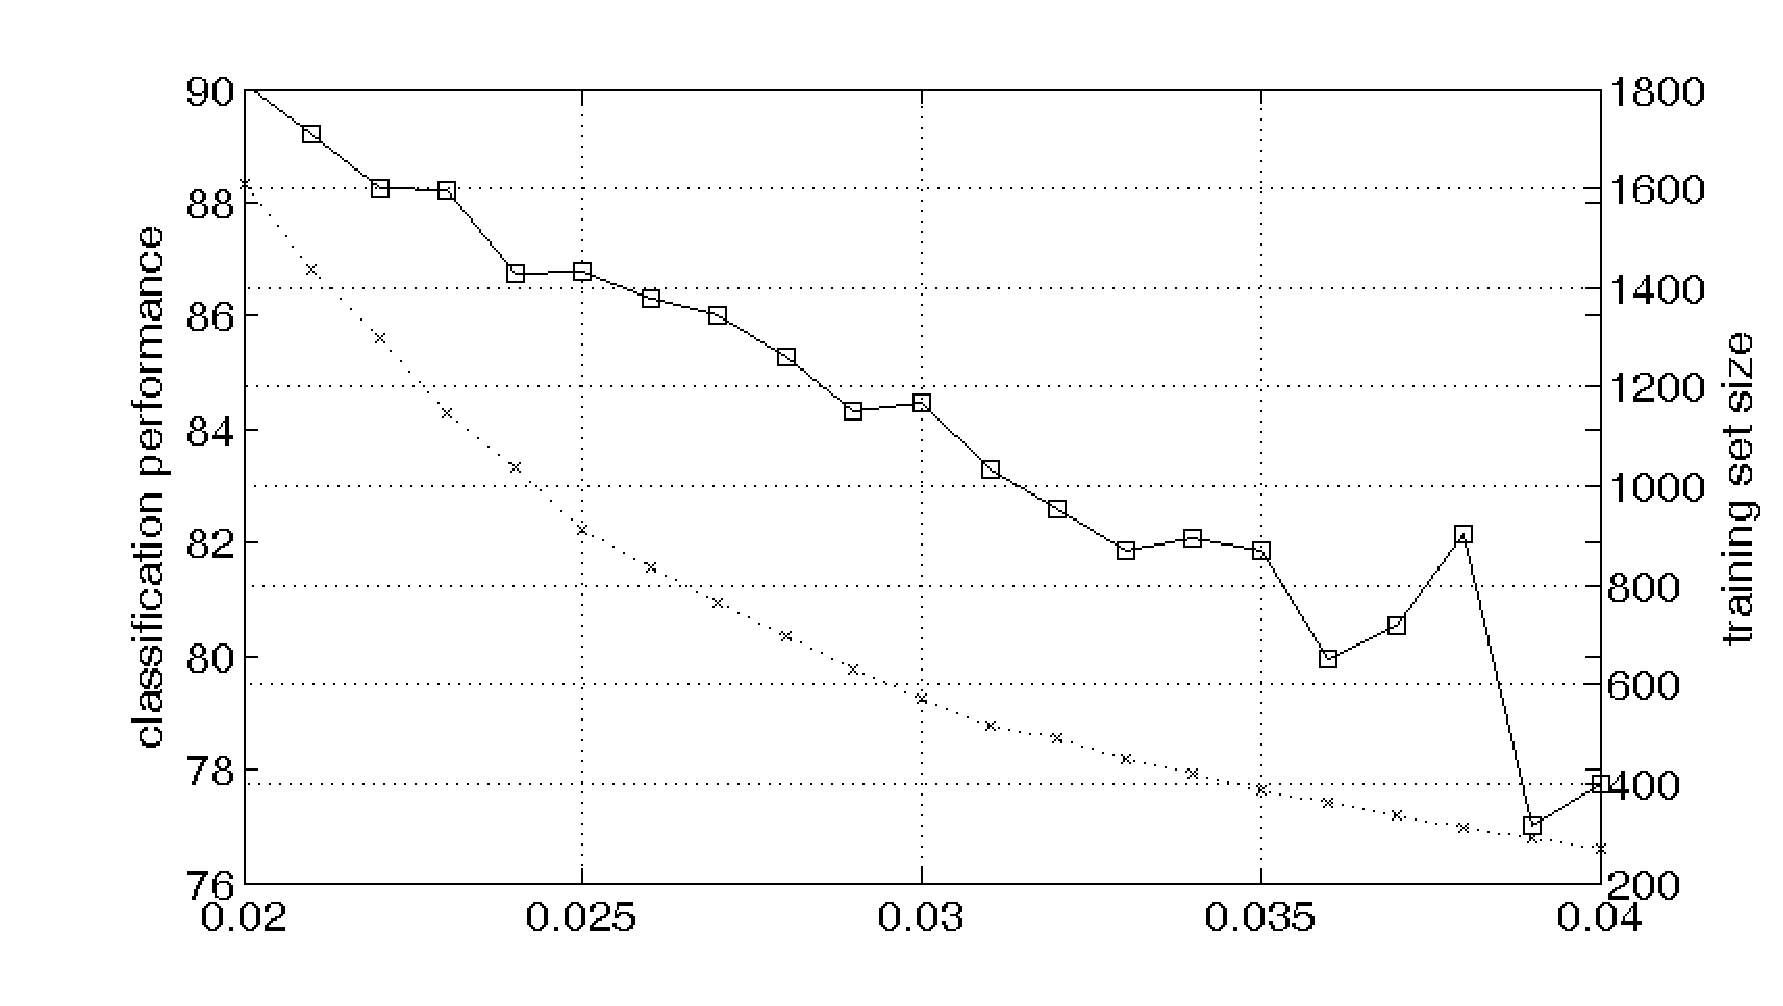
\includegraphics[width=0.6\textwidth]{subj8.eps} \\
%  \end{tabular}
  \caption{size of the training set (dotted line) and classification
    performance (continuous line), of subject $8$ in the FA phase, as
    $d$ changes.}
  \label{fig:subj8}
\end{figure}

\begin{figure}[!ht] \centering
%  \begin{tabular}{cc}
%    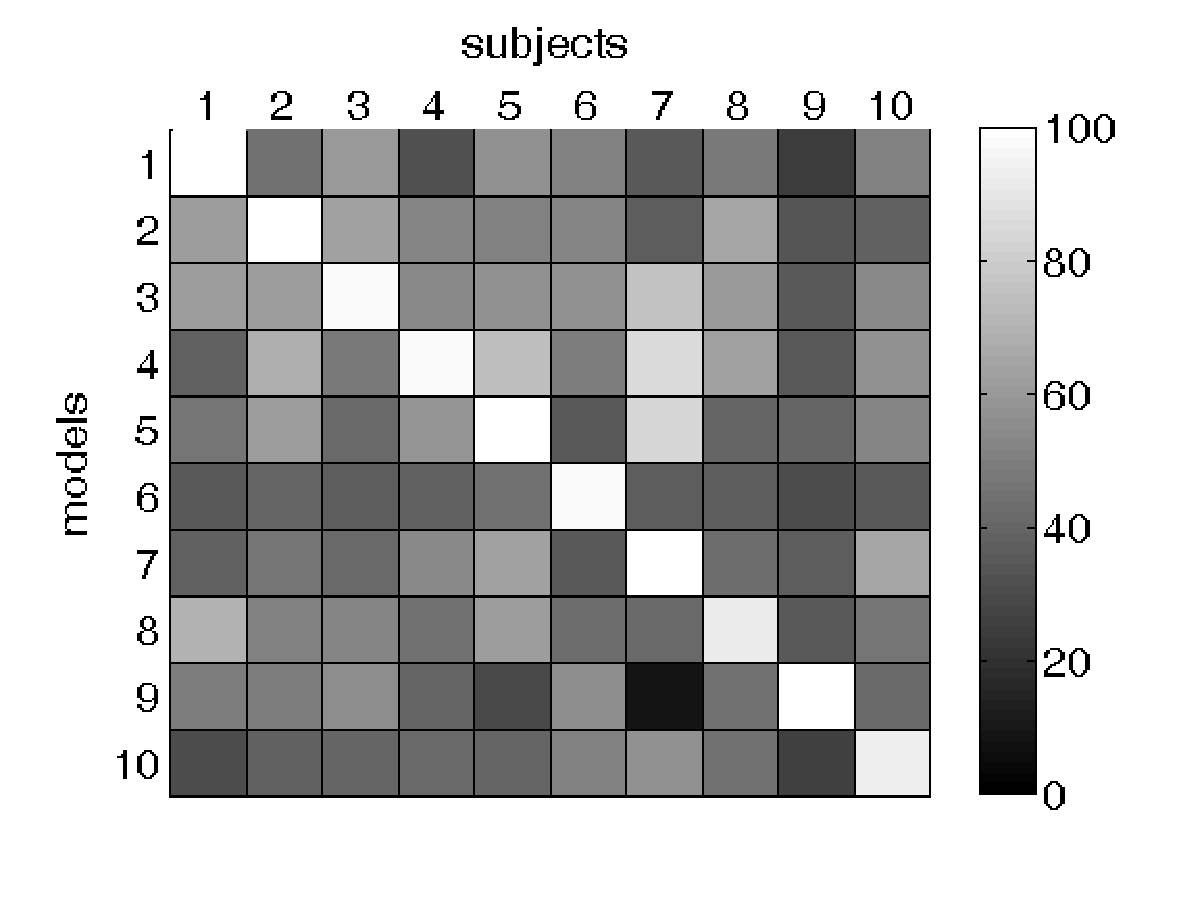
\includegraphics[width=0.45\textwidth]{crossClass1.eps} & \includegraphics[width=0.45\textwidth]{crossClass2.eps} \\
%    $51.69\% \pm 19.27\%$ & $54.04\% \pm 16.42\%$ \\
%    \includegraphics[width=0.45\textwidth]{crossRegr1.eps} & \includegraphics[width=0.45\textwidth]{crossRegr2.eps} \\
%    $0.60 \pm 0.18$ & $0.58 \pm 0.19$ \\
%  \end{tabular}
  \caption{cross-subject performance matrices, for classification (top
    row) and regression (bottom row), in the SA (left column)
    and FA phase (right column); the numbers refer to all element of
    the matrices, excluding the diagonals.}
  \label{fig:cross}
\end{figure}

\end{bmcformat}

\end{document}
